\chapter{Raw Data Figures}
\label{sec:appendix_b}

\section{Exploratory Stocks Data Graphs}
\label{sec:stock_ohlc}
The figures below depict combined line graphs of the opening, high, low, and 
closing prices of each stock in the alamSYS. These figures also demonstrate why 
closing prices were chosen as the primary training feature of the models developed 
for this particular problem. Aside from being the most important price target in most 
trading and investing strategies, closing prices do not differ significantly from the 
other price metrics.

% AC
\begin{figure}[ht]
    \centering
    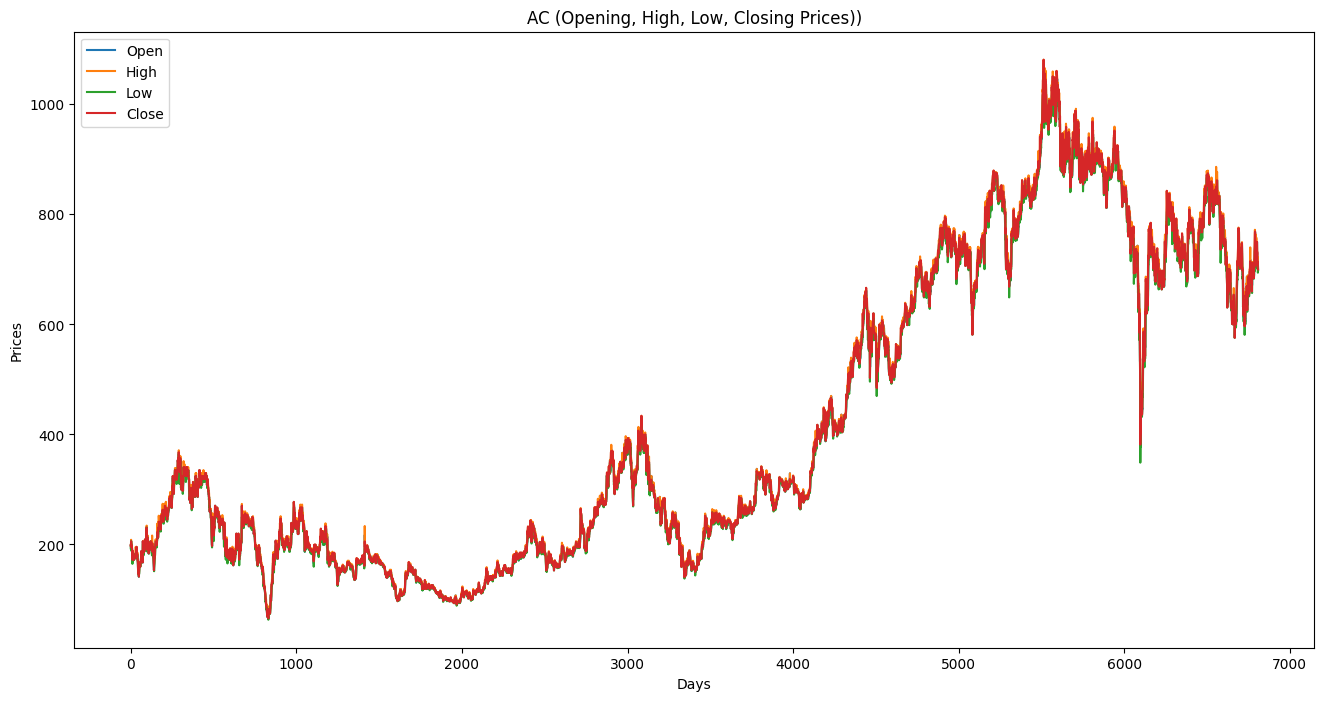
\includegraphics[width=0.80\textwidth]{./assets/Appendices/B/OHLC_Prices/AC.png}
    \caption{Opening, High, Low, and Closing Prices on AC}
    \label{fig:ohlc_AC}
\end{figure}
\FloatBarrier
    
% ALI
\begin{figure}[ht]
    \centering
    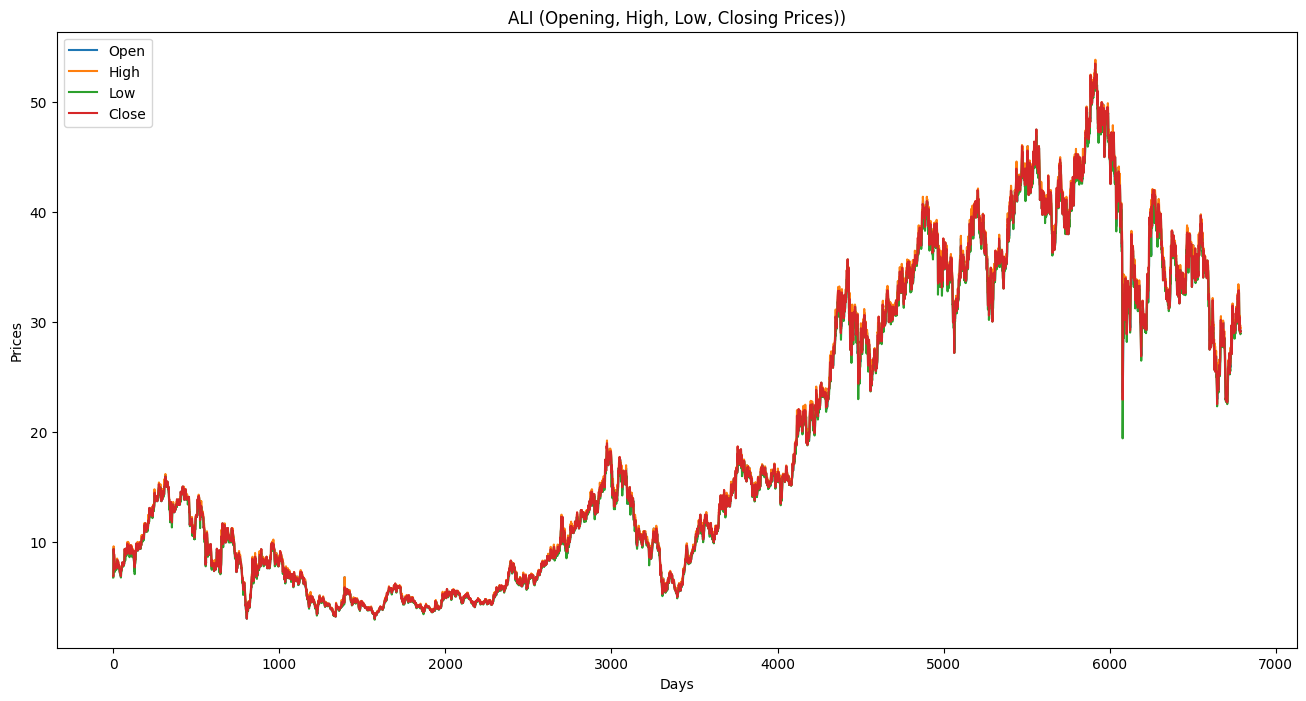
\includegraphics[width=0.80\textwidth]{./assets/Appendices/B/OHLC_Prices/ALI.png}
    \caption{Opening, High, Low, and Closing Prices for ALI}
    \label{fig:ohlc_ALI}
\end{figure}
\FloatBarrier

% AP
\begin{figure}[ht]
    \centering
    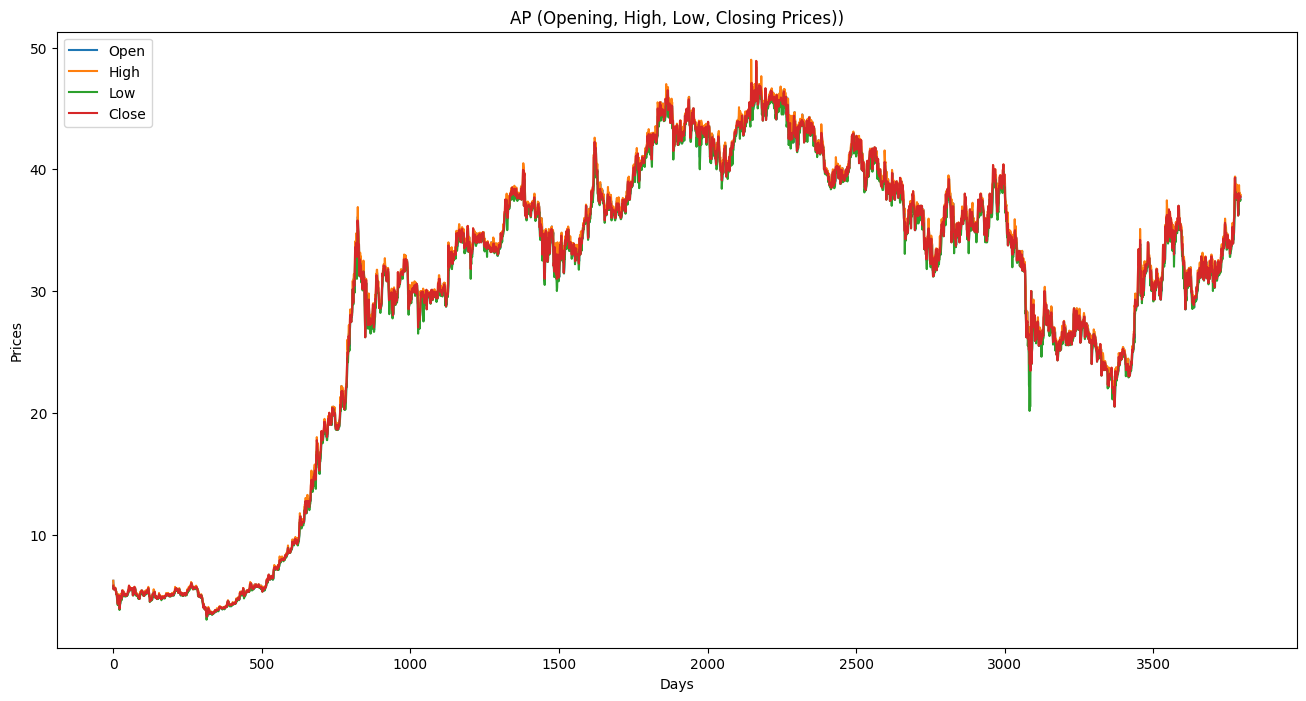
\includegraphics[width=0.80\textwidth]{./assets/Appendices/B/OHLC_Prices/AP.png}
    \caption{Opening, High, Low, and Closing Prices for AP}
    \label{fig:ohlc_AP}
\end{figure}
\FloatBarrier

% BDO
\begin{figure}[ht]
    \centering
    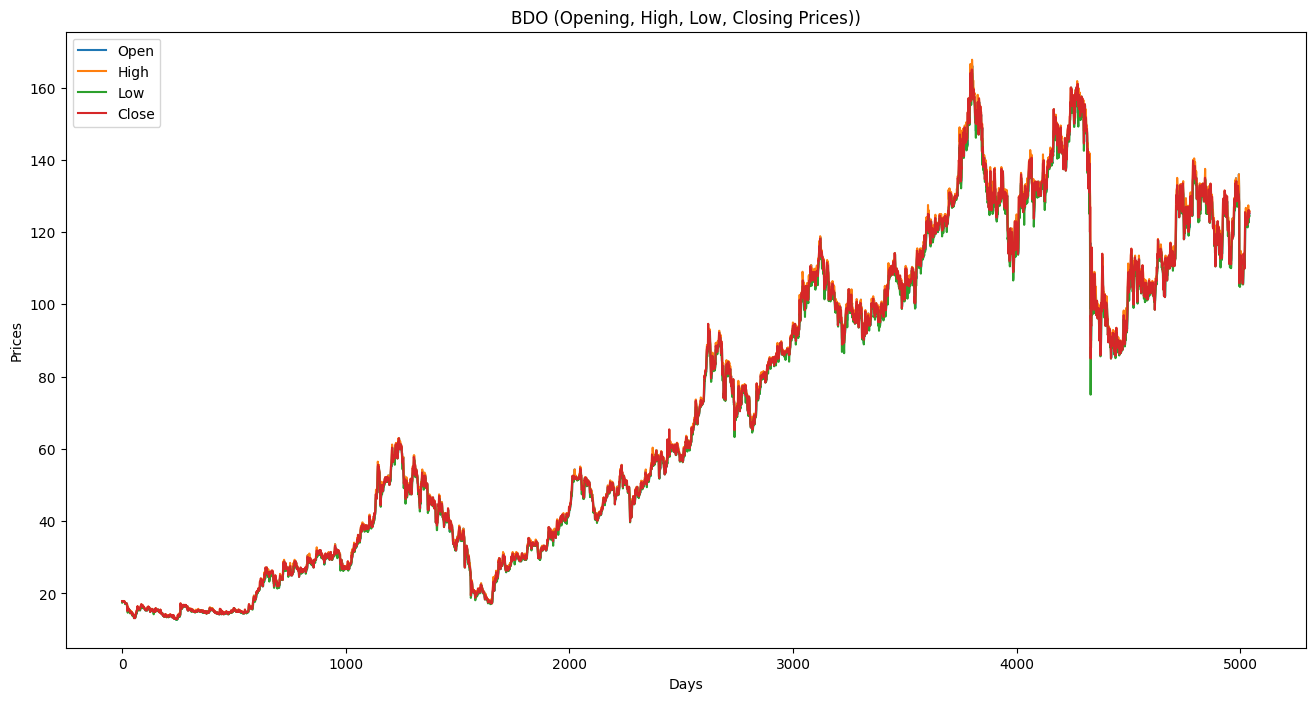
\includegraphics[width=0.80\textwidth]{./assets/Appendices/B/OHLC_Prices/BDO.png}
    \caption{Opening, High, Low, and Closing Prices for BDO}
    \label{fig:ohlc_BDO}
\end{figure}
\FloatBarrier

% BLOOM
\begin{figure}[ht]
    \centering
    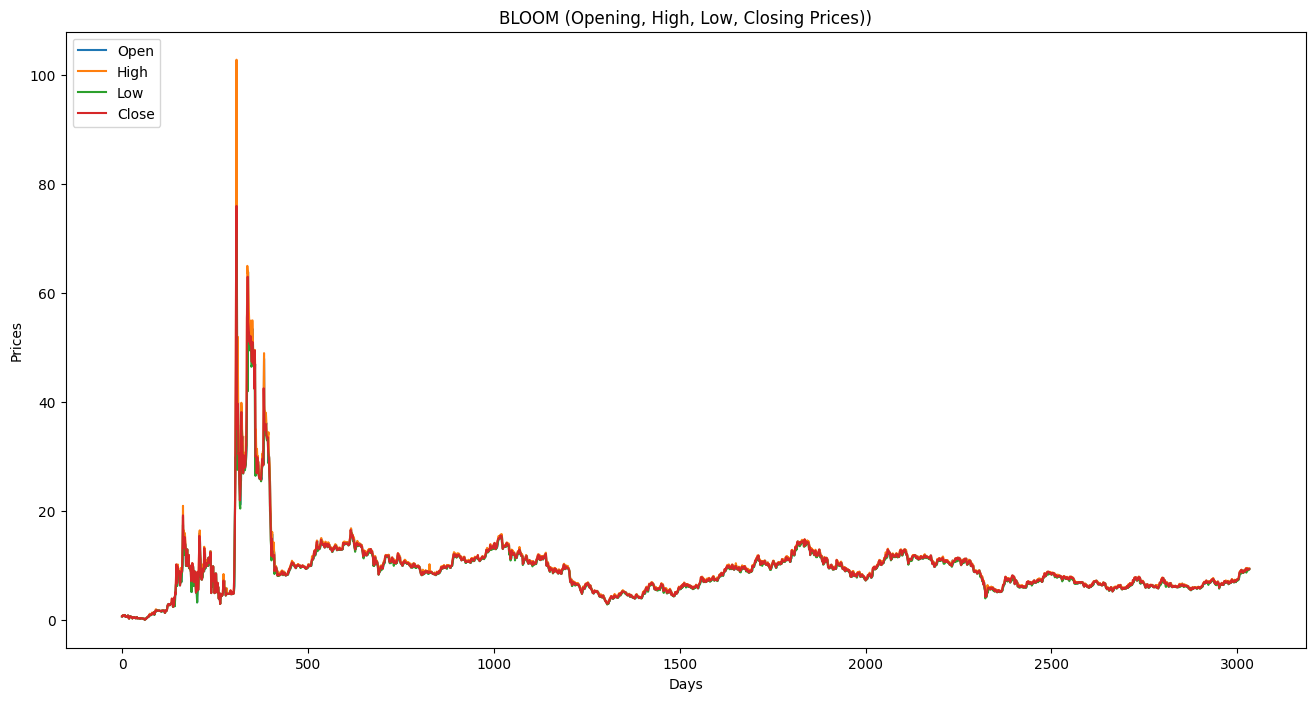
\includegraphics[width=0.80\textwidth]{./assets/Appendices/B/OHLC_Prices/BLOOM.png}
    \caption{Opening, High, Low, and Closing Prices for BLOOM}
    \label{fig:ohlc_BLOOM}
\end{figure}
\FloatBarrier

% FGEN
\begin{figure}[ht]
    \centering
    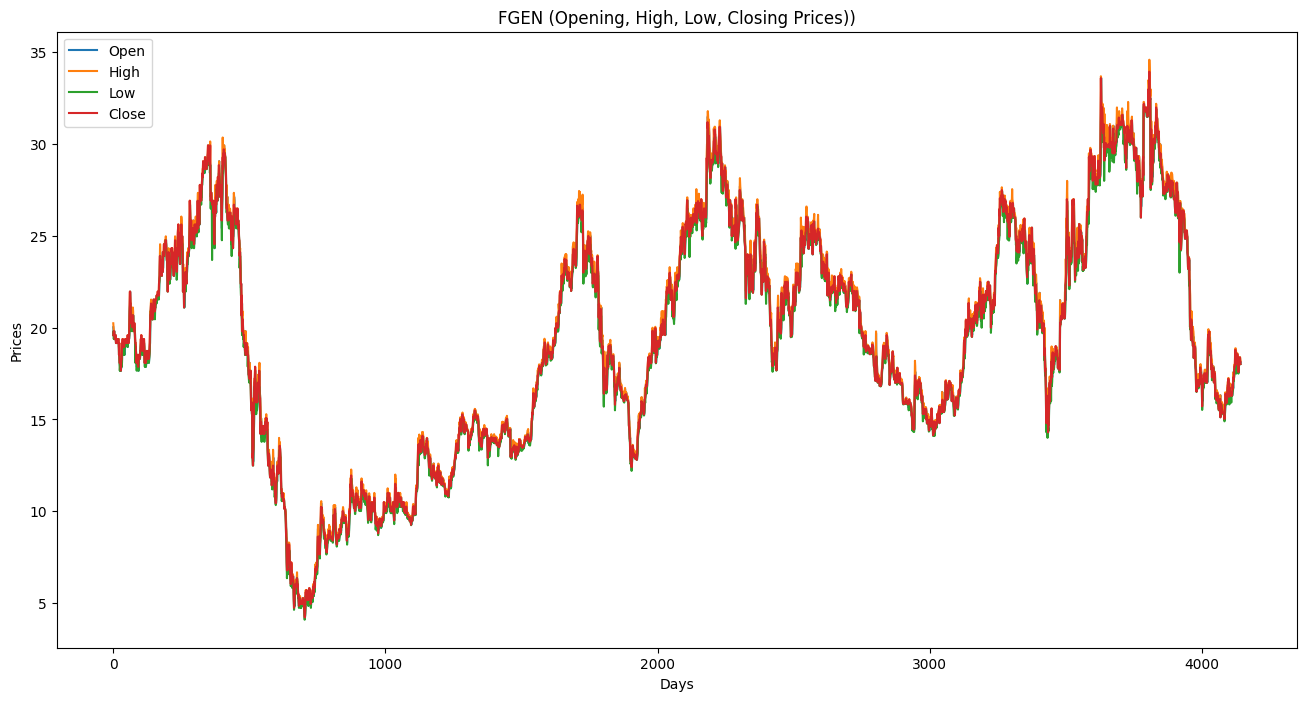
\includegraphics[width=0.80\textwidth]{./assets/Appendices/B/OHLC_Prices/FGEN.png}
    \caption{Opening, High, Low, and Closing Prices for FGEN}
    \label{fig:ohlc_FGEN}
\end{figure}
\FloatBarrier

% GLO
\begin{figure}[ht]
    \centering
    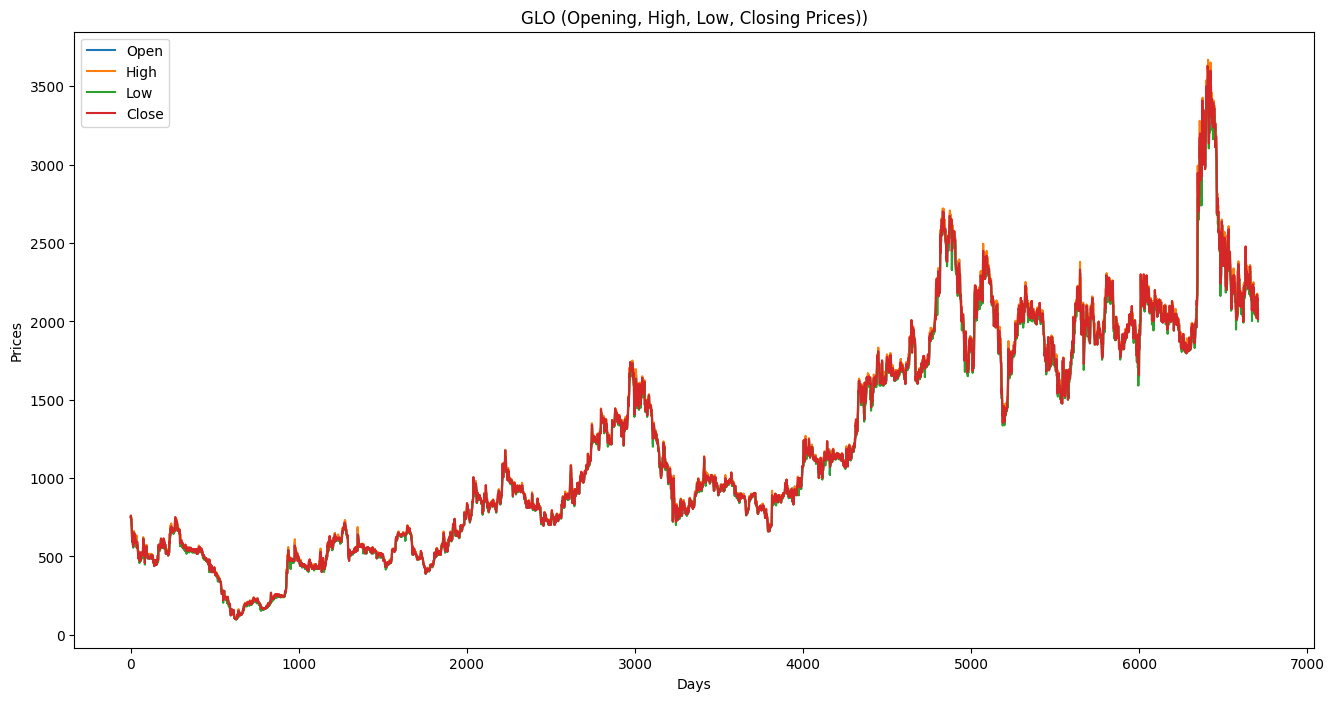
\includegraphics[width=0.80\textwidth]{./assets/Appendices/B/OHLC_Prices/GLO.png}
    \caption{Opening, High, Low, and Closing Prices for GLO}
    \label{fig:ohlc_GLO}
\end{figure}
\FloatBarrier

% ICT
\begin{figure}[ht]
    \centering
    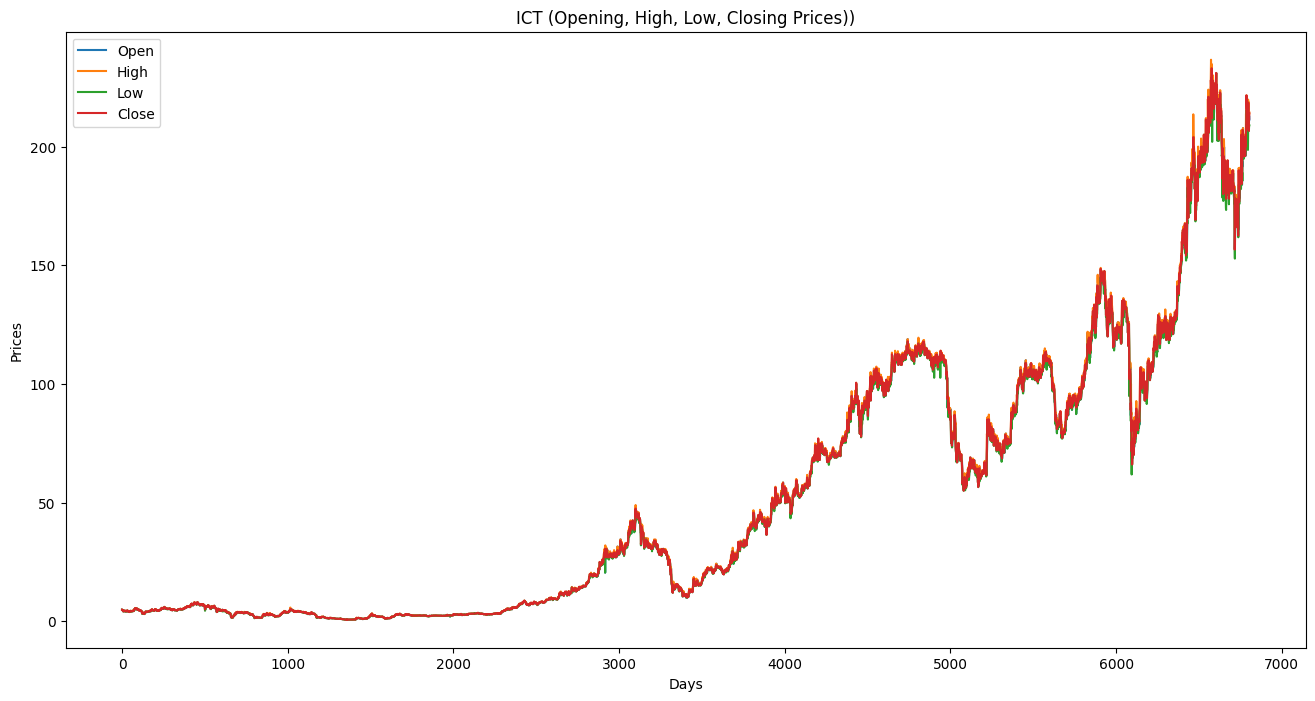
\includegraphics[width=0.80\textwidth]{./assets/Appendices/B/OHLC_Prices/ICT.png}
    \caption{Opening, High, Low, and Closing Prices for ICT}
    \label{fig:ohlc_ICT}
\end{figure}
\FloatBarrier

% JGS
\begin{figure}[ht]
    \centering
    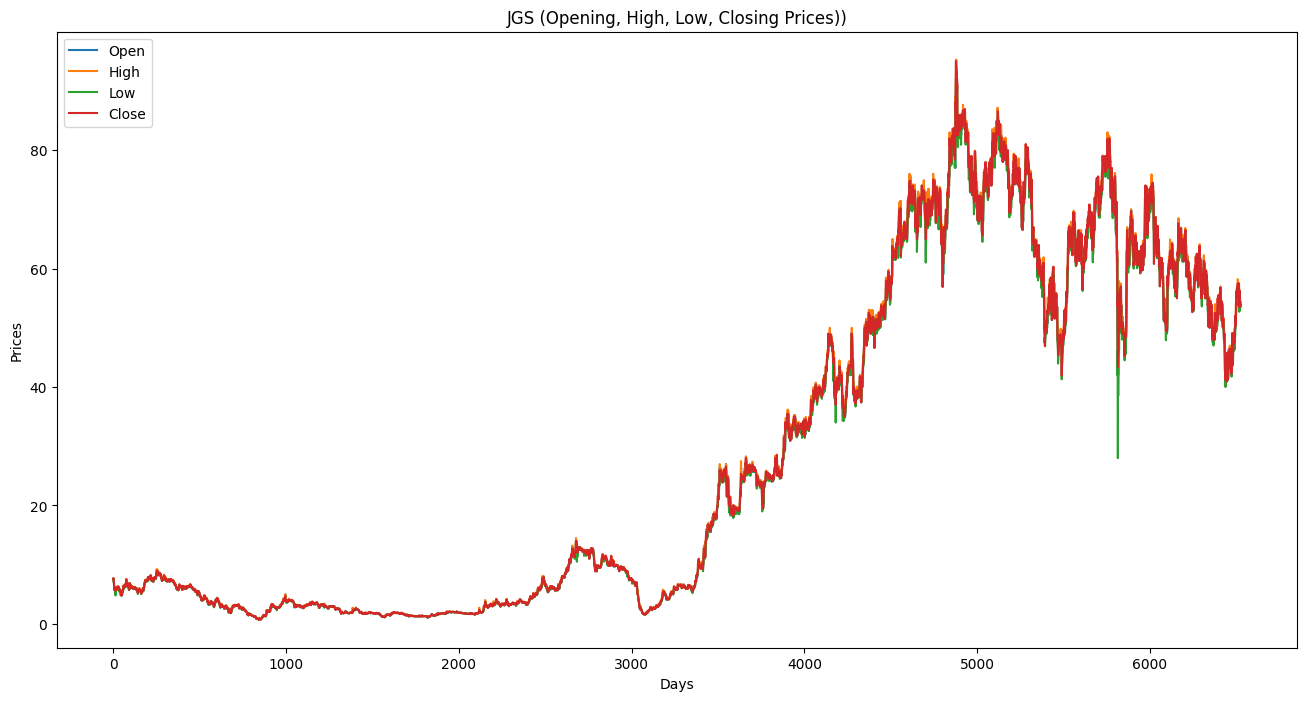
\includegraphics[width=0.80\textwidth]{./assets/Appendices/B/OHLC_Prices/JGS.png}
    \caption{Opening, High, Low, and Closing Prices on JGS}
    \label{fig:ohlc_JGS}
\end{figure}
\FloatBarrier
    
% LTG
\begin{figure}[ht]
    \centering
    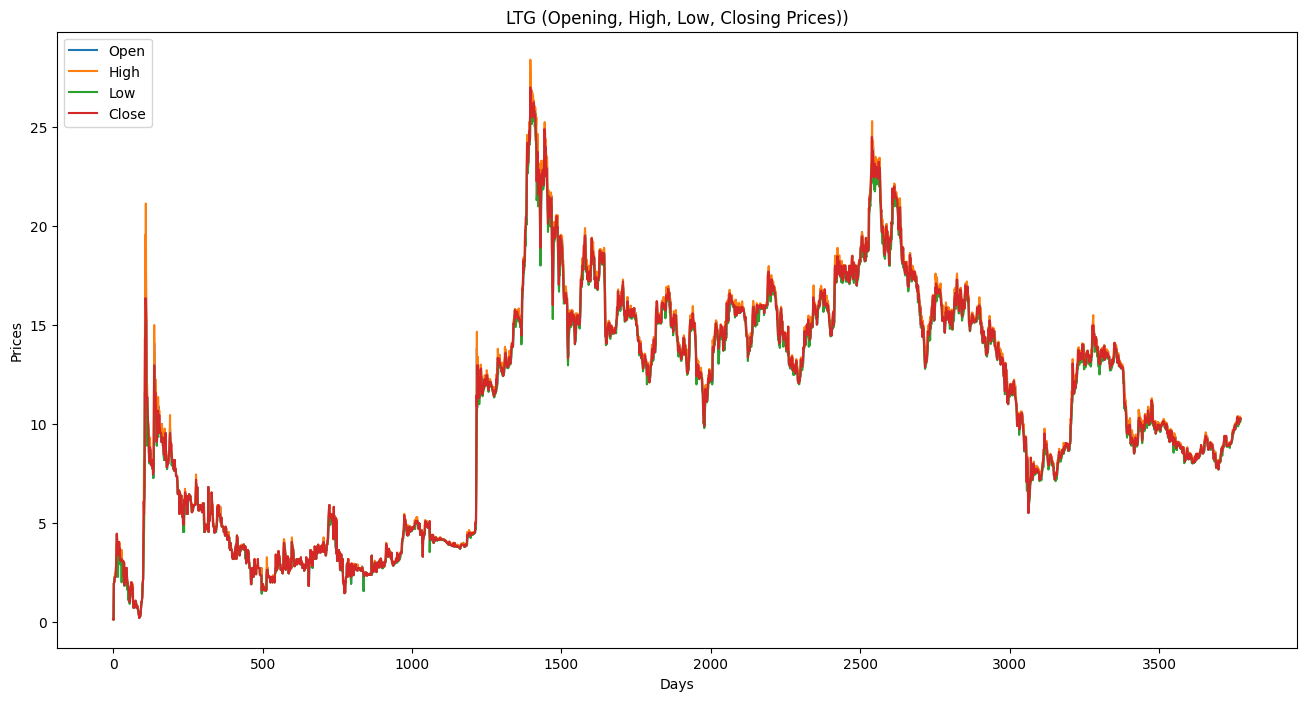
\includegraphics[width=0.80\textwidth]{./assets/Appendices/B/OHLC_Prices/LTG.png}
    \caption{Opening, High, Low, and Closing Prices on LTG}
    \label{fig:ohlc_LTG}
\end{figure}
\FloatBarrier

% MEG
\begin{figure}[ht]
    \centering
    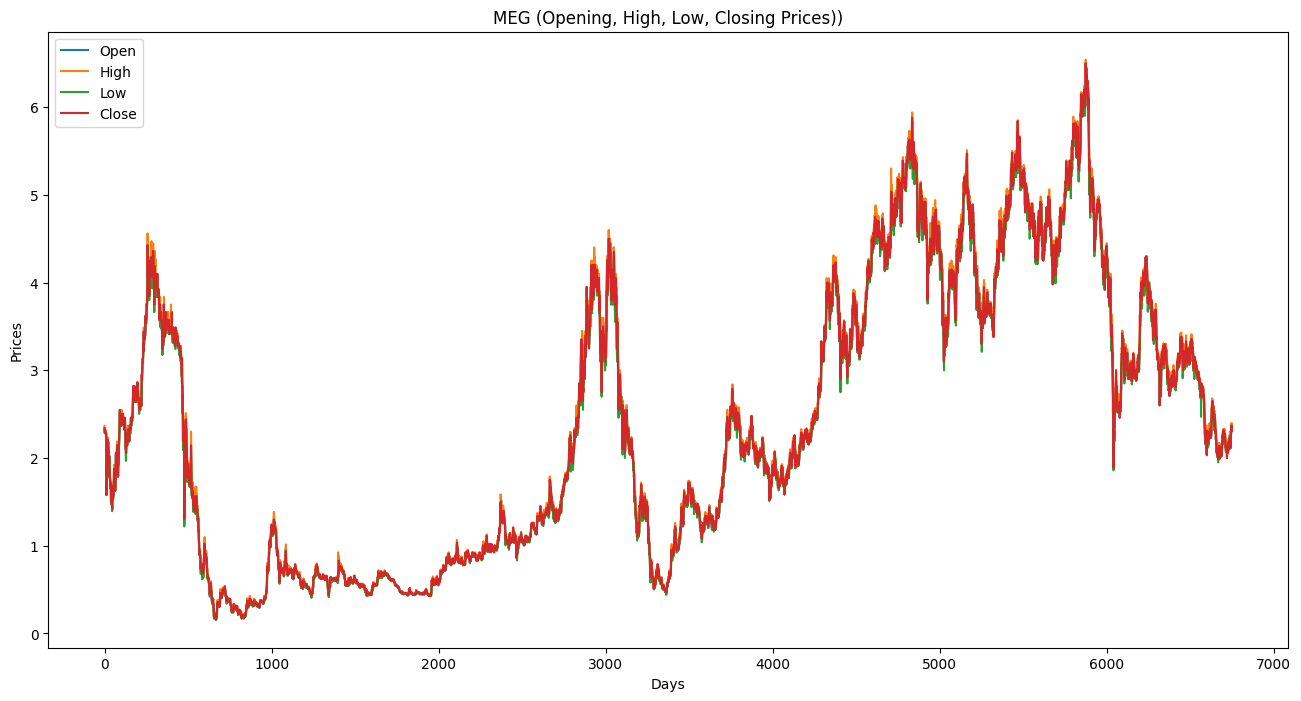
\includegraphics[width=0.80\textwidth]{./assets/Appendices/B/OHLC_Prices/MEG.png}
    \caption{Opening, High, Low, and Closing Prices on MEG}
    \label{fig:ohlc_MEG}
\end{figure}
\FloatBarrier

% MER
\begin{figure}[ht]
    \centering
    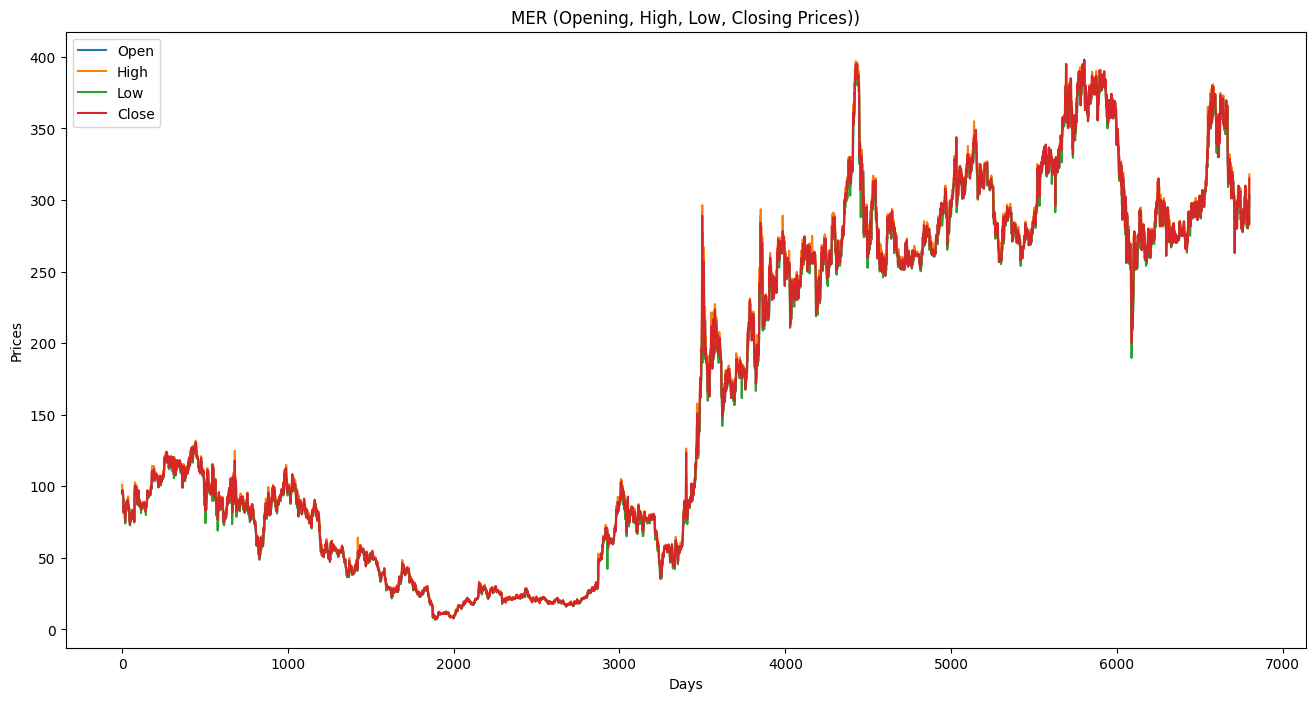
\includegraphics[width=0.80\textwidth]{./assets/Appendices/B/OHLC_Prices/MER.png}
    \caption{Opening, High, Low, and Closing Prices on MER}
    \label{fig:ohlc_MER}
\end{figure}
\FloatBarrier

% MPI
\begin{figure}[ht]
    \centering
    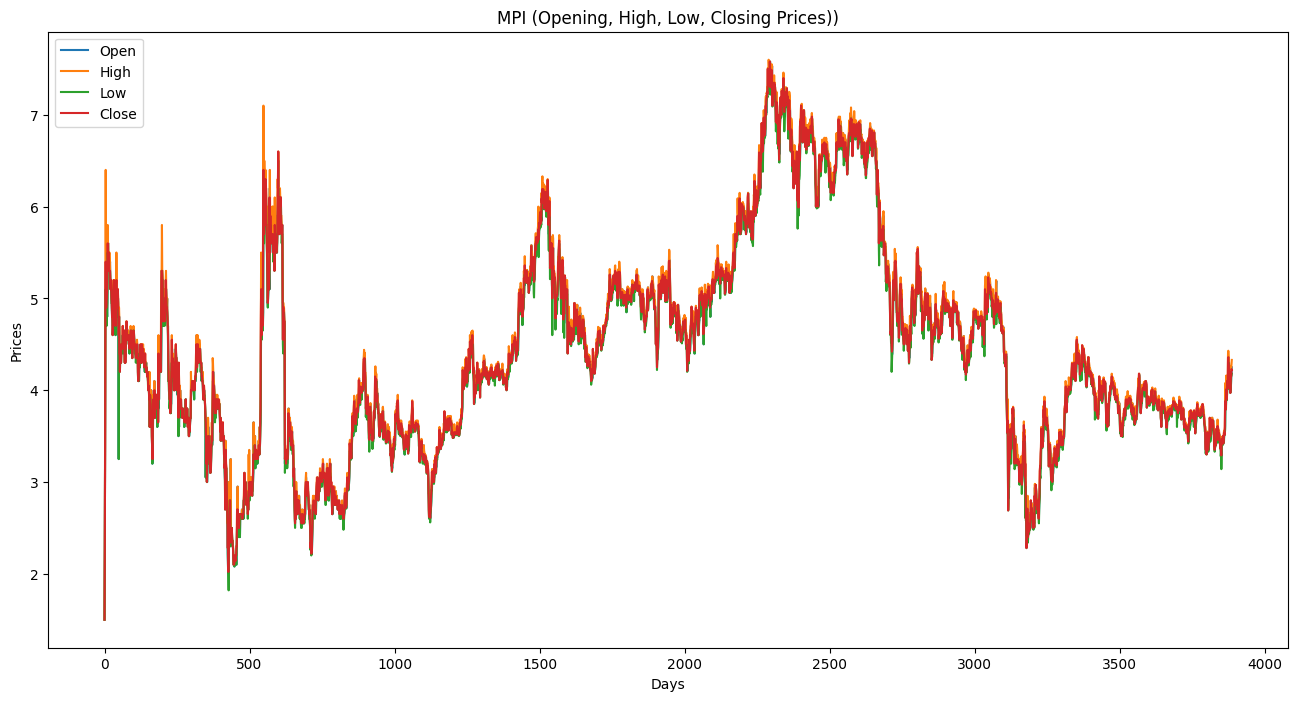
\includegraphics[width=0.80\textwidth]{./assets/Appendices/B/OHLC_Prices/MPI.png}
    \caption{Opening, High, Low, and Closing Prices on MPI}
    \label{fig:ohlc_MPI}
\end{figure}
\FloatBarrier

% PGOLD
\begin{figure}[ht]
    \centering
    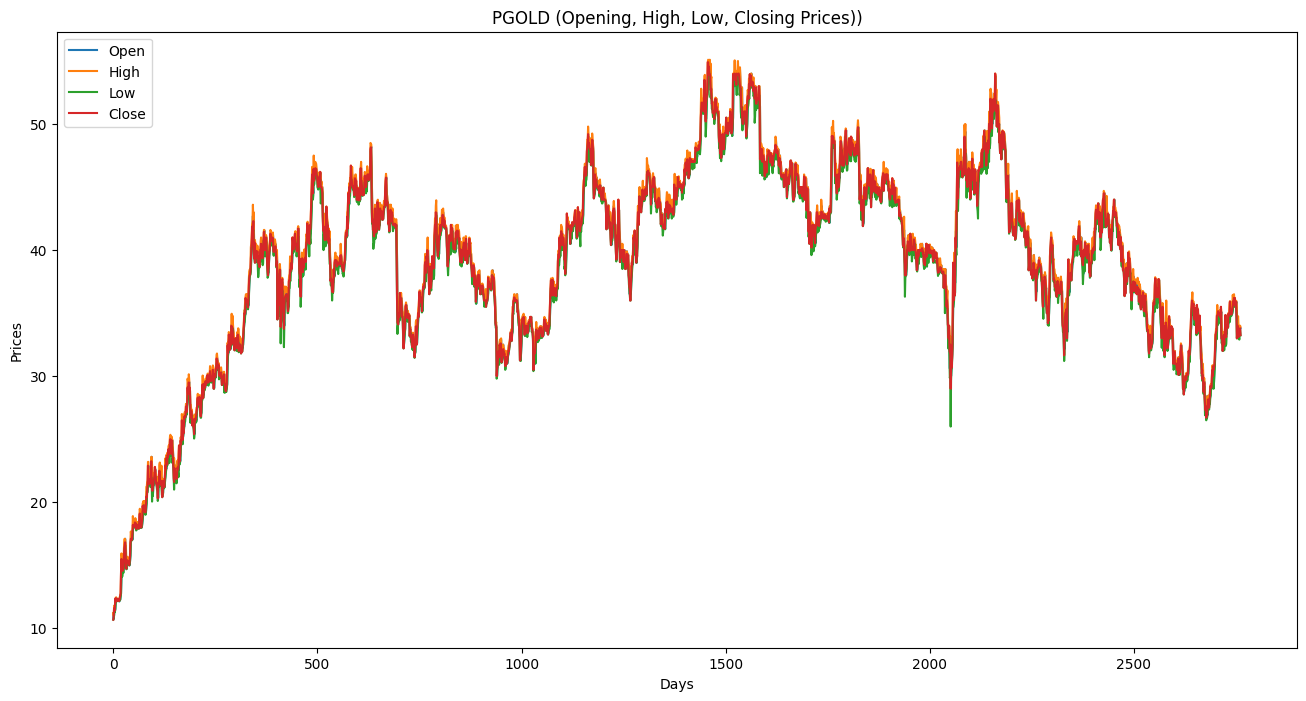
\includegraphics[width=0.80\textwidth]{./assets/Appendices/B/OHLC_Prices/PGOLD.png}
    \caption{Opening, High, Low, and Closing Prices on PGOLD}
    \label{fig:ohlc_PGOLD}
\end{figure}
\FloatBarrier

% PSEI
\begin{figure}[ht]
    \centering
    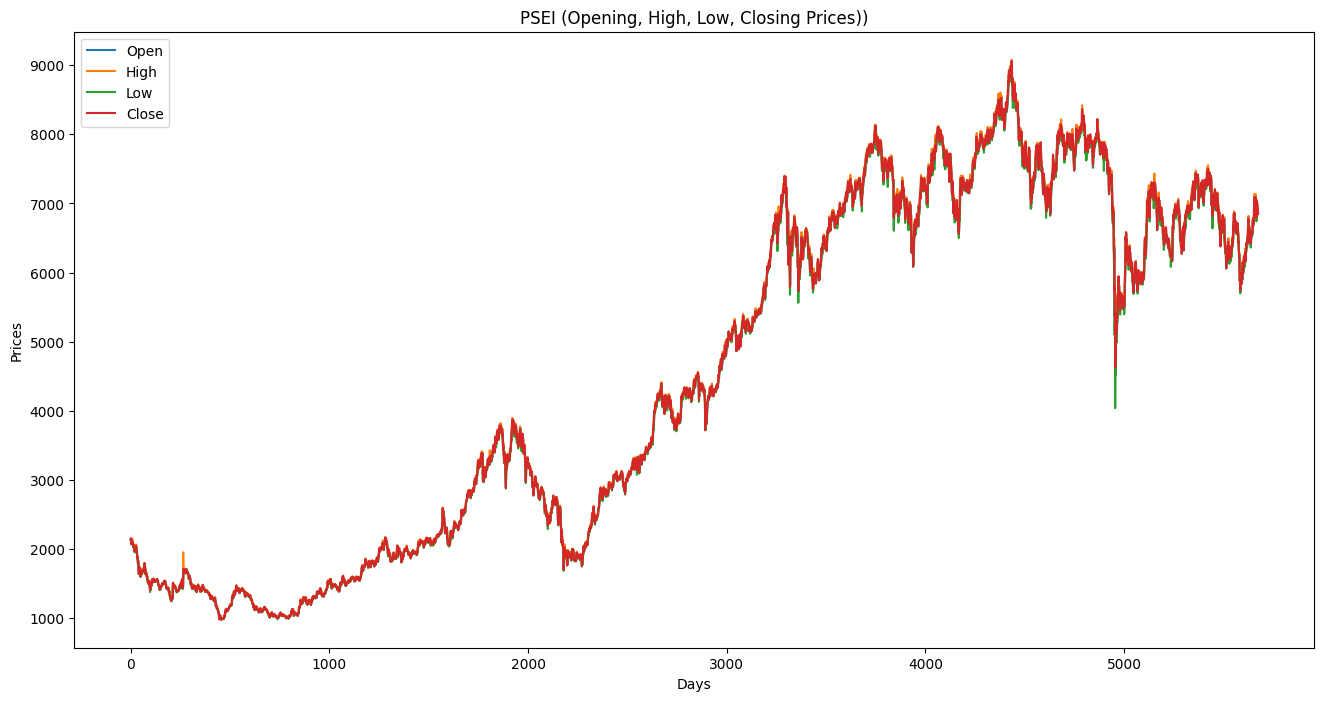
\includegraphics[width=0.80\textwidth]{./assets/Appendices/B/OHLC_Prices/PSEI.png}
    \caption{Opening, High, Low, and Closing Prices on PSEI}
    \label{fig:ohlc_PSEI}
\end{figure}
\FloatBarrier

% RLC
\begin{figure}[ht]
    \centering
    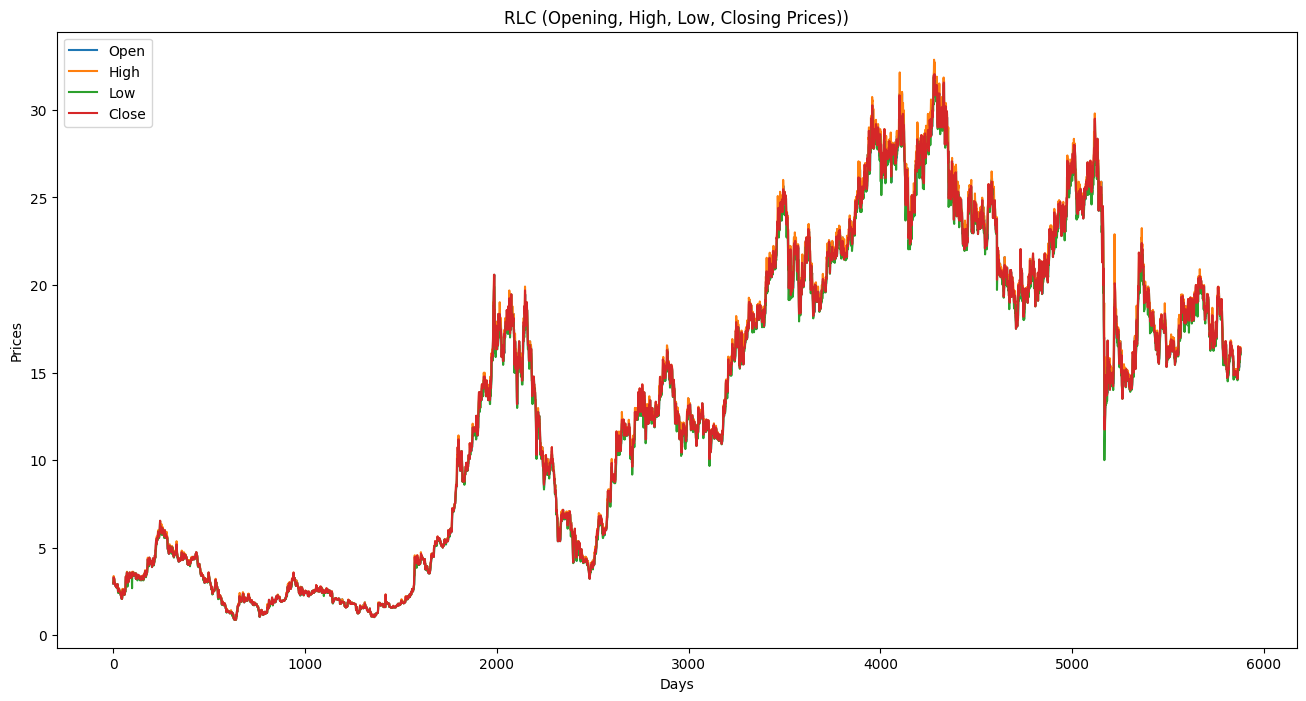
\includegraphics[width=0.80\textwidth]{./assets/Appendices/B/OHLC_Prices/RLC.png}
    \caption{Opening, High, Low, and Closing Prices on RLC}
    \label{fig:ohlc_RLC}
\end{figure}
\FloatBarrier

% RRHI
\begin{figure}[ht]
    \centering
    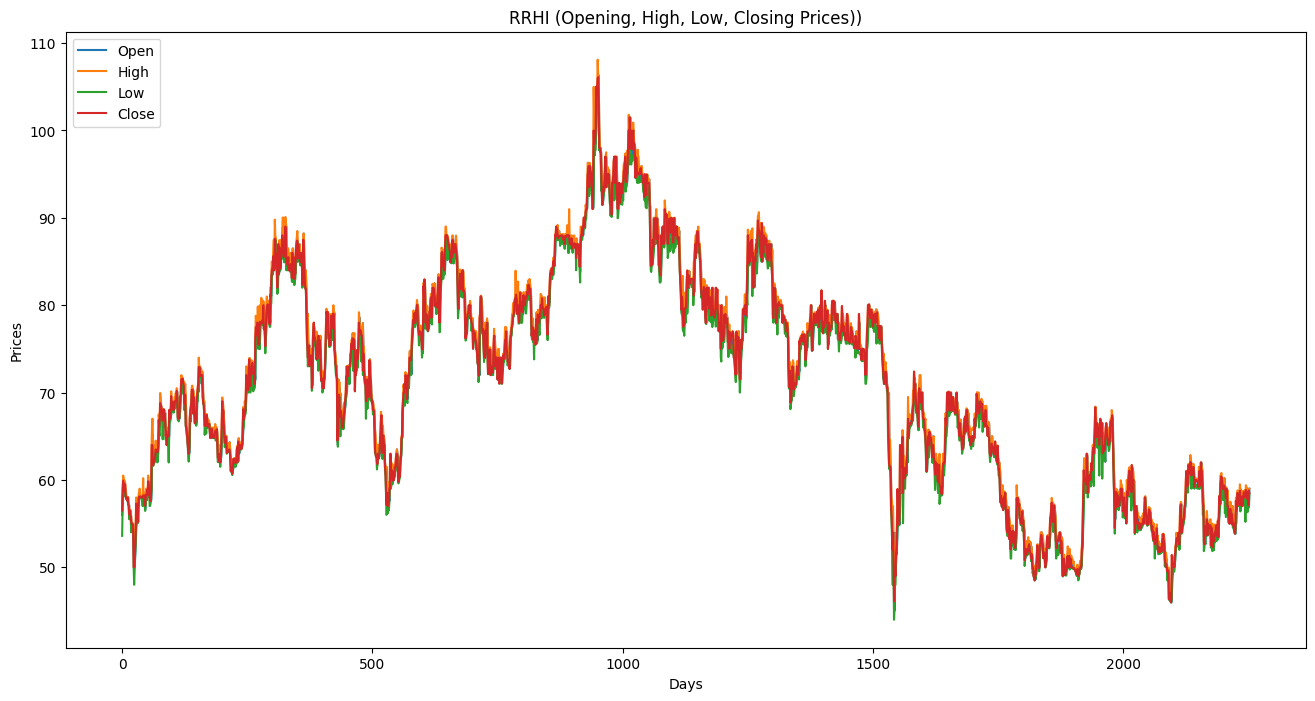
\includegraphics[width=0.80\textwidth]{./assets/Appendices/B/OHLC_Prices/RRHI.png}
    \caption{Opening, High, Low, and Closing Prices on RRHI}
    \label{fig:ohlc_RRHI}
\end{figure}
\FloatBarrier

% SMC
\begin{figure}[ht]
    \centering
    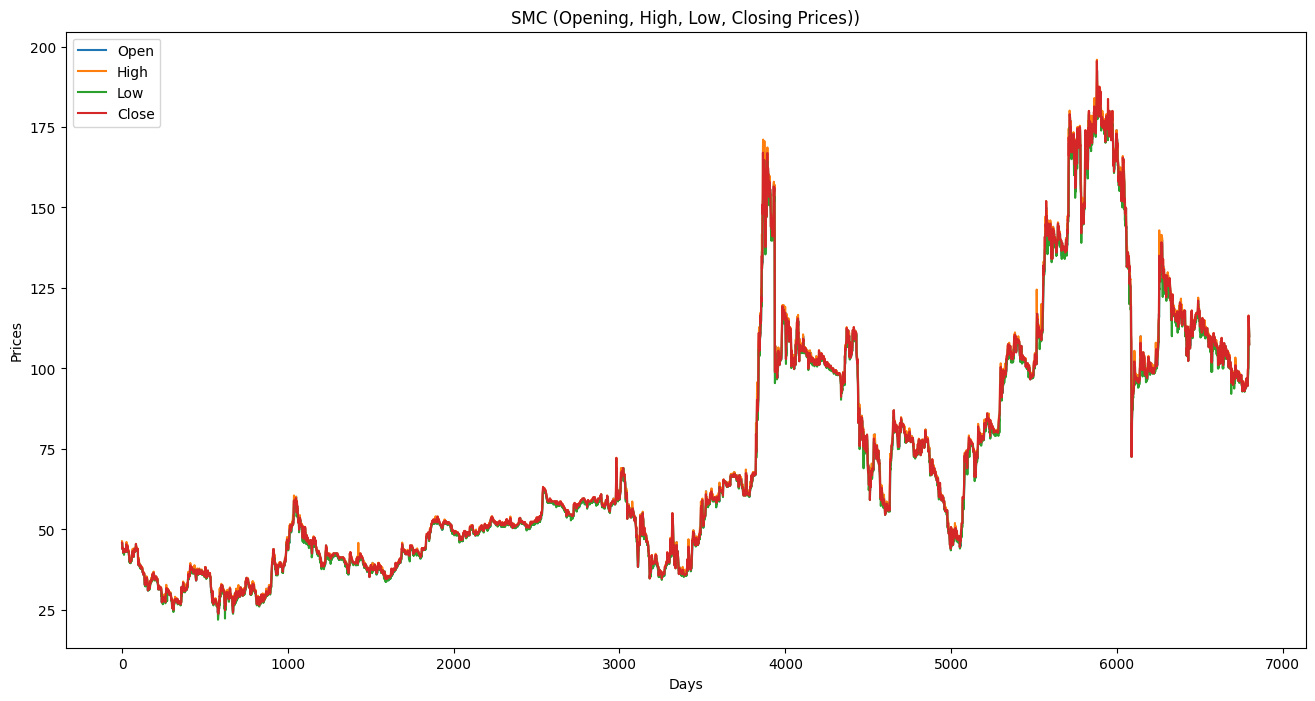
\includegraphics[width=0.80\textwidth]{./assets/Appendices/B/OHLC_Prices/SMC.png}
    \caption{Opening, High, Low, and Closing Prices on SMC}
    \label{fig:ohlc_SMC}
\end{figure}
\FloatBarrier

% TEL
\begin{figure}[ht]
    \centering
    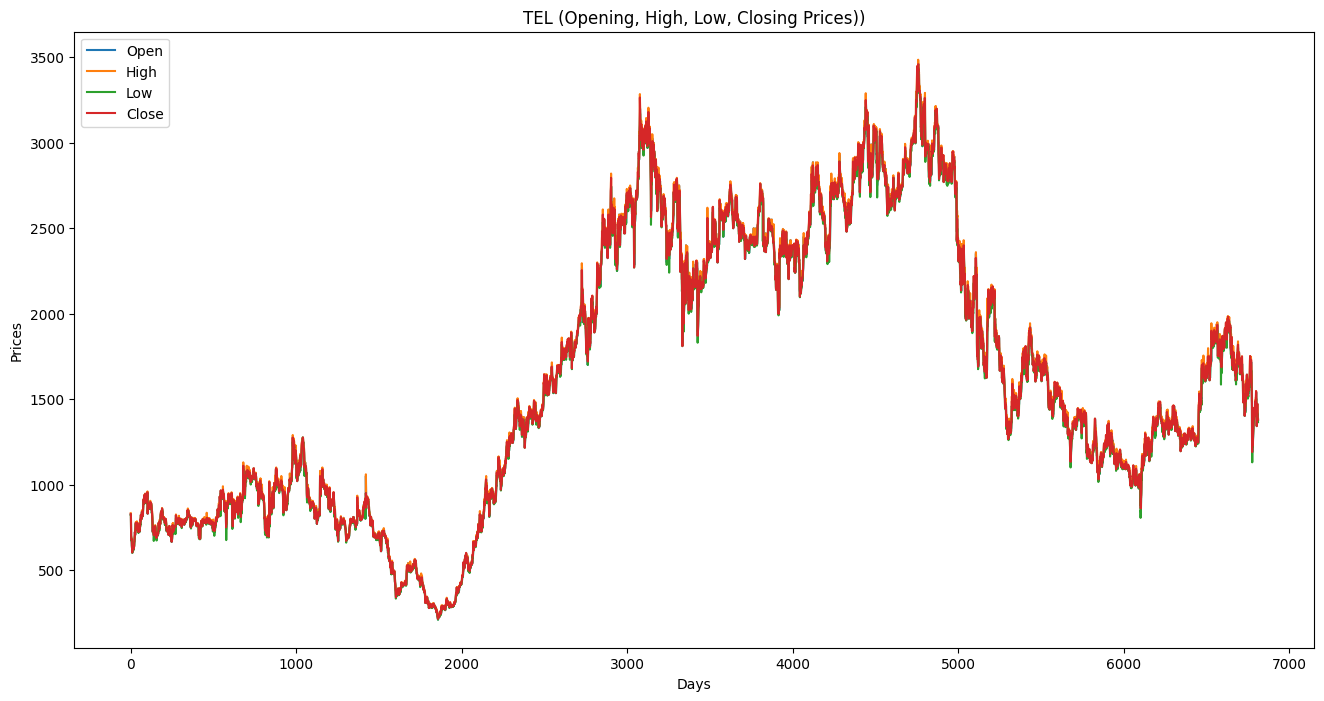
\includegraphics[width=0.80\textwidth]{./assets/Appendices/B/OHLC_Prices/TEL.png}
    \caption{Opening, High, Low, and Closing Prices on TEL}
    \label{fig:ohlc_TEL}
\end{figure}
\FloatBarrier

% URC
\begin{figure}[ht]
    \centering
    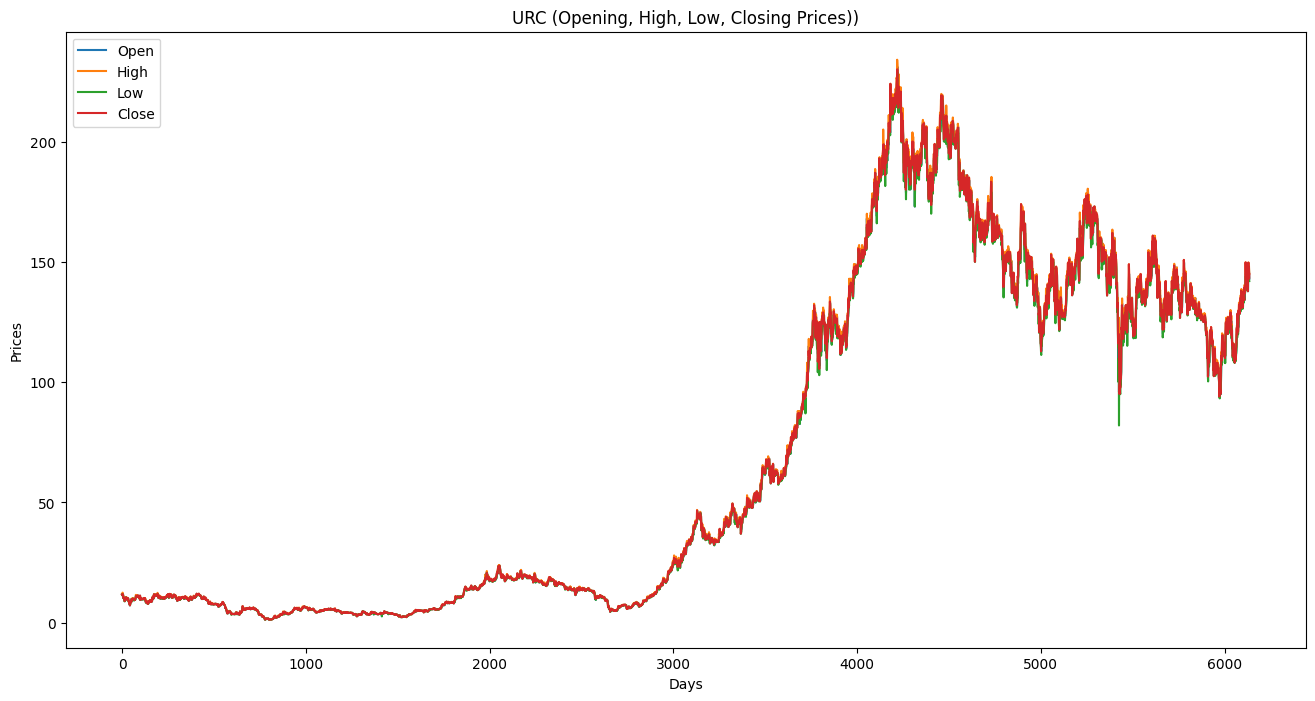
\includegraphics[width=0.80\textwidth]{./assets/Appendices/B/OHLC_Prices/URC.png}
    \caption{Opening, High, Low, and Closing Prices on URC}
    \label{fig:ohlc_URC}
\end{figure}
\FloatBarrier


\section{Raw Model Testing and Cross-Validation Results}
The loss metric scores for all eight models trained in this special problem are shown in the 
figures below.

% baseline5
\begin{figure}[ht]
    \centering
    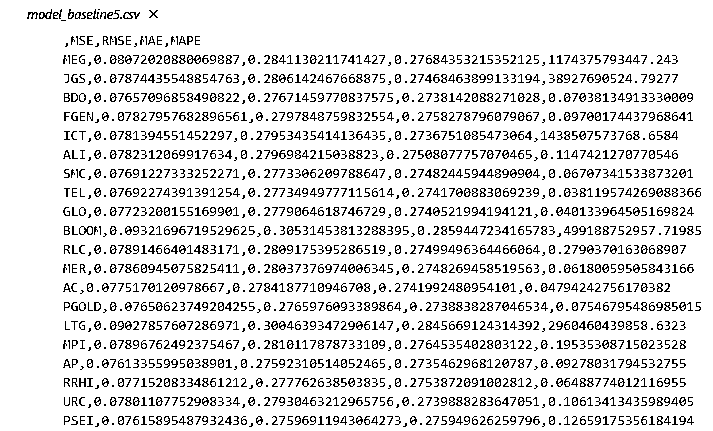
\includegraphics[width=0.80\textwidth]{./assets/Appendices/B/RawScores/baseline5.png}
    \caption{Raw Model Scores for Baseline 5}
    \label{fig:rawScores_baseline5}
\end{figure}
\FloatBarrier

% baseline10
\begin{figure}[ht]
    \centering
    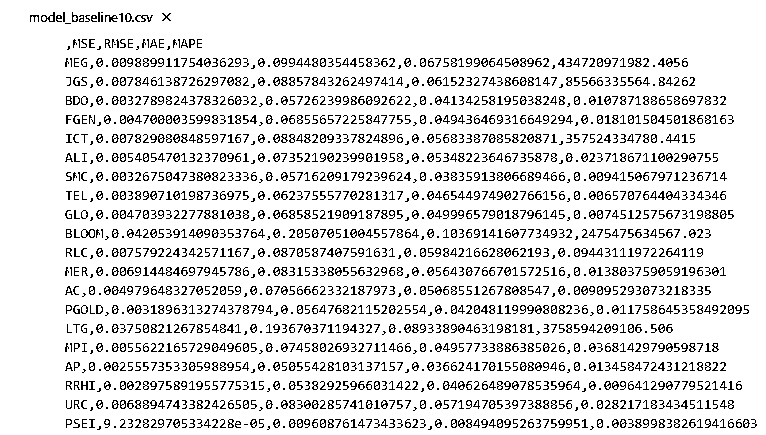
\includegraphics[width=0.80\textwidth]{./assets/Appendices/B/RawScores/baseline10.png}
    \caption{Raw Model Scores for Baseline 10}
    \label{fig:rawScores_baseline10}
\end{figure}
\FloatBarrier

% baseline15
\begin{figure}[ht]
    \centering
    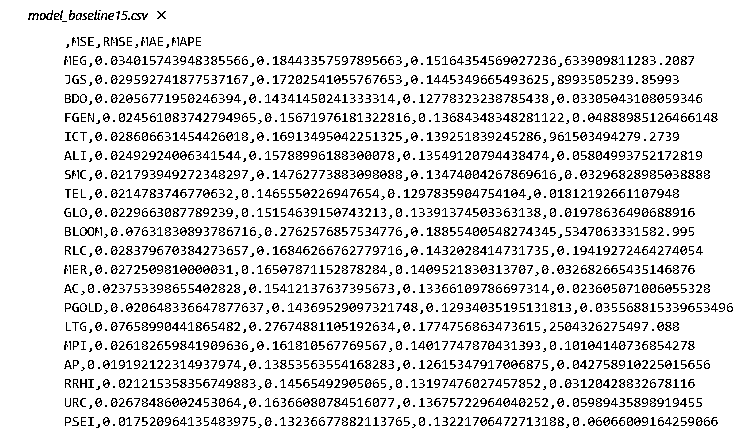
\includegraphics[width=0.80\textwidth]{./assets/Appendices/B/RawScores/baseline15.png}
    \caption{Raw Model Scores for Baseline 15}
    \label{fig:rawScores_baseline15}
\end{figure}
\FloatBarrier

% baseline20
\begin{figure}[ht]
    \centering
    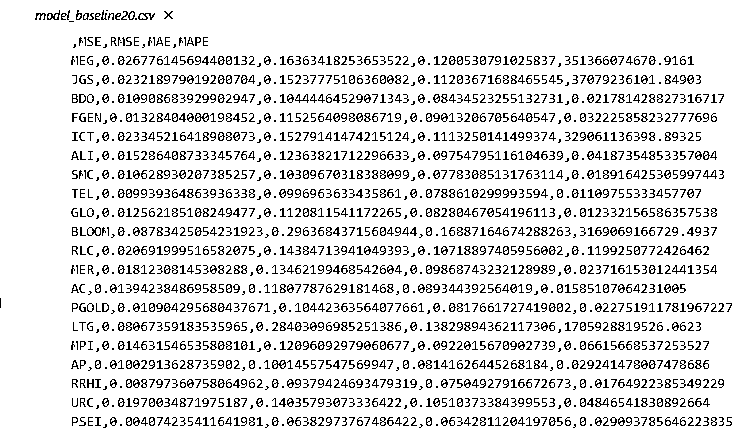
\includegraphics[width=0.80\textwidth]{./assets/Appendices/B/RawScores/baseline20.png}
    \caption{Raw Model Scores for Baseline 20}
    \label{fig:rawScores_baseline20}
\end{figure}
\FloatBarrier

% dmd_lstm5
\begin{figure}[ht]
    \centering
    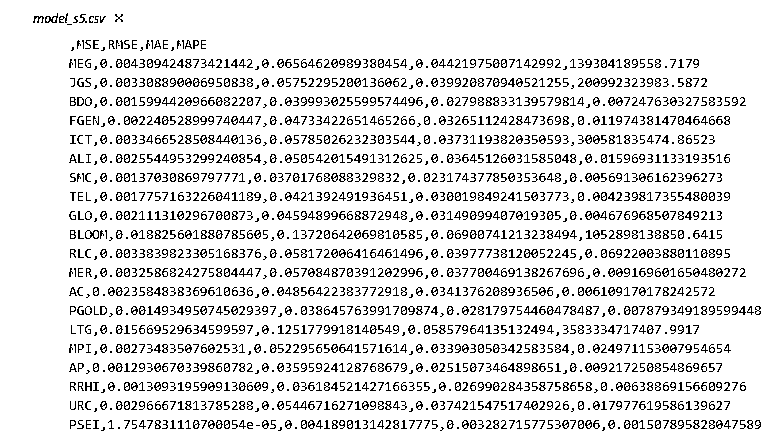
\includegraphics[width=0.80\textwidth]{./assets/Appendices/B/RawScores/dmdlstm5.png}
    \caption{Raw Model Scores for DMD-LSTM 5}
    \label{fig:rawScores_dmdlstm5}
\end{figure}
\FloatBarrier

% dmdlstm10
\begin{figure}[ht]
    \centering
    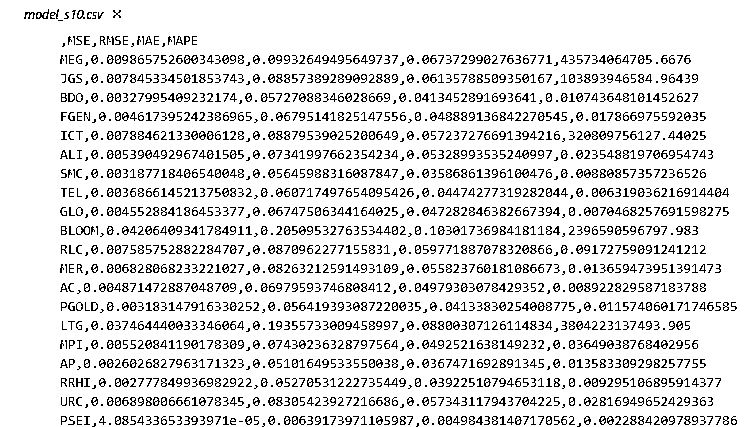
\includegraphics[width=0.80\textwidth]{./assets/Appendices/B/RawScores/dmdlstm10.png}
    \caption{Raw Model Scores for DMD-LSTM 10}
    \label{fig:rawScores_dmdlstm10}
\end{figure}
\FloatBarrier

% dmdlstm15
\begin{figure}[ht]
    \centering
    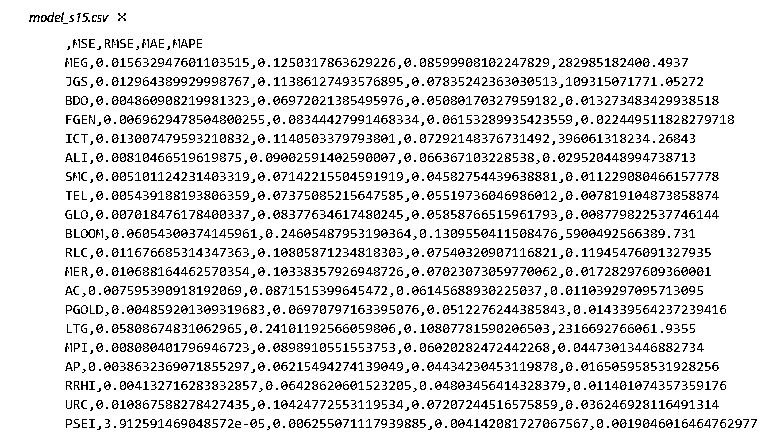
\includegraphics[width=0.80\textwidth]{./assets/Appendices/B/RawScores/dmdlstm15.png}
    \caption{Raw Model Scores for DMD-LSTM 15}
    \label{fig:rawScores_dmdlstm15}
\end{figure}
\FloatBarrier

% dmdlstm20
\begin{figure}[ht]
    \centering
    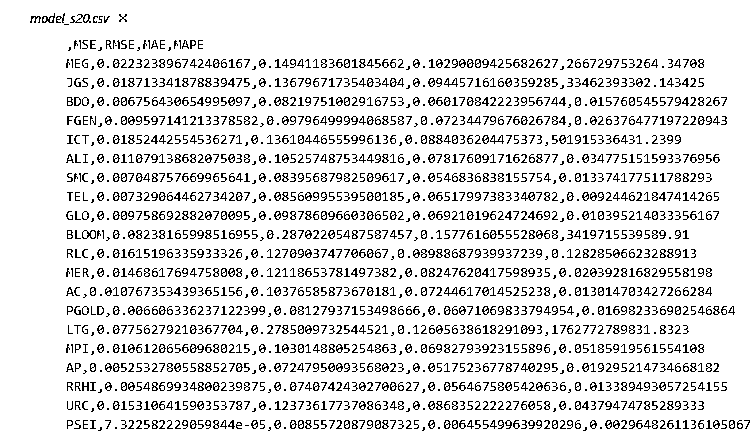
\includegraphics[width=0.80\textwidth]{./assets/Appendices/B/RawScores/dmdlstm20.png}
    \caption{Raw Model Scores for DMD-LSTM 20}
    \label{fig:rawScores_dmdlstm20}
\end{figure}
\FloatBarrier


\section{Model Testing Raw Test Results for DMD-LSTM}
\label{sec:raw_test_dmd-lstm}
The graphs below show the performance of the different DMD-LSTM models 
trained in the conduct of this special problem based on the test data split of PSEI.

% dmd_lstm5
\begin{figure}[ht]
    \centering
    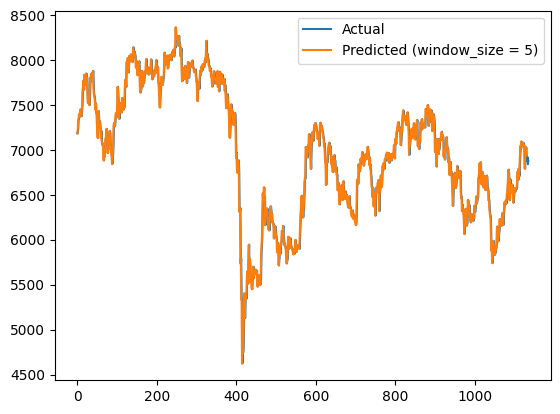
\includegraphics[width=0.80\textwidth]{./assets/Appendices/B/Model_Testing/dmd_lstm5.png}
    \caption{Actual vs Predicted Closing Prices for DMD-LSTM 5 (Using Train Data from PSEI)}
    \label{fig:modelTest_dmd_lstm5}
\end{figure}
\FloatBarrier

% dmd_lstm10
\begin{figure}[ht]
    \centering
    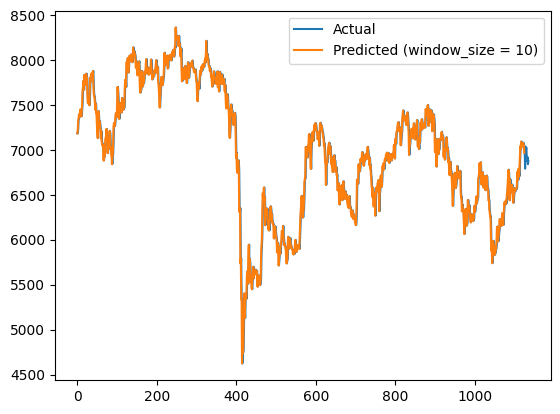
\includegraphics[width=0.80\textwidth]{./assets/Appendices/B/Model_Testing/dmd_lstm10.png}
    \caption{Actual vs Predicted Closing Prices for DMD-LSTM 10 (Using Train Data from PSEI)}
    \label{fig:modelTest_dmd_lstm10}
\end{figure}
\FloatBarrier

% dmd_lstm15
\begin{figure}[ht]
    \centering
    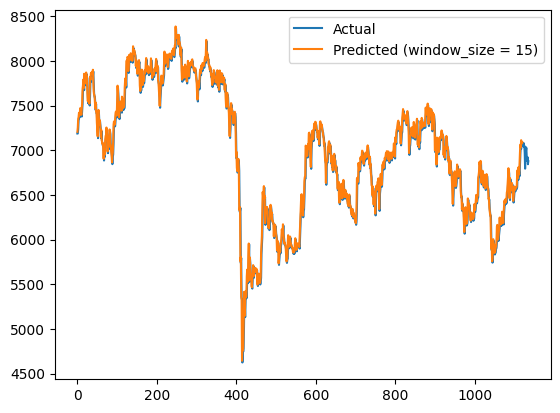
\includegraphics[width=0.80\textwidth]{./assets/Appendices/B/Model_Testing/dmd_lstm15.png}
    \caption{Actual vs Predicted Closing Prices for DMD-LSTM 15 (Using Train Data from PSEI)}
    \label{fig:modelTest_dmd_lstm15}
\end{figure}
\FloatBarrier

% dmd_lstm20
\begin{figure}[ht]
    \centering
    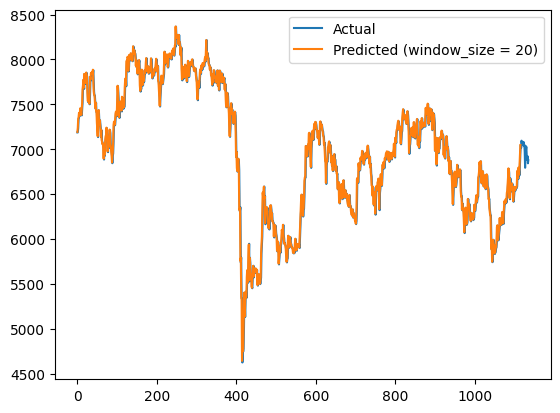
\includegraphics[width=0.80\textwidth]{./assets/Appendices/B/Model_Testing/dmd_lstm20.png}
    \caption{Actual vs Predicted Closing Prices for DMD-LSTM 20 (Using Train Data from PSEI)}
    \label{fig:modelTest_dmd_lstm20}
\end{figure}
\FloatBarrier


\section{Daily Return Distribution of the Different Stocks}
\label{sec:daily_return_distribution}
Figures below show the daily return distribution of each stock, which was used to 
calculate each stock's risk profile.

% AC
\begin{figure}[ht]
    \centering
    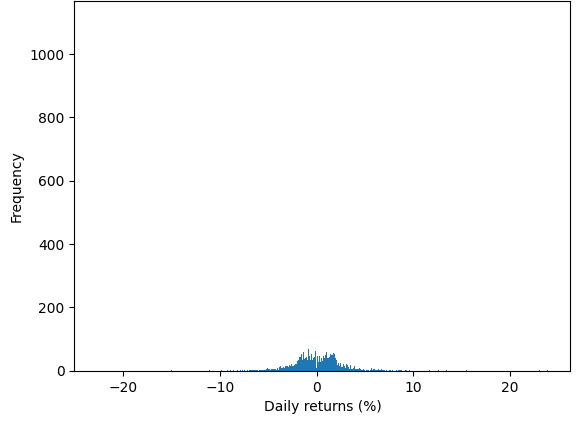
\includegraphics[width=0.80\textwidth]{./assets/Appendices/B/Distribution_DailyReturns/AC.png}
    \caption{Daily Return Distribution of AC}
    \label{fig:returndist_AC}
\end{figure}
\FloatBarrier
    
% ALI
\begin{figure}[ht]
    \centering
    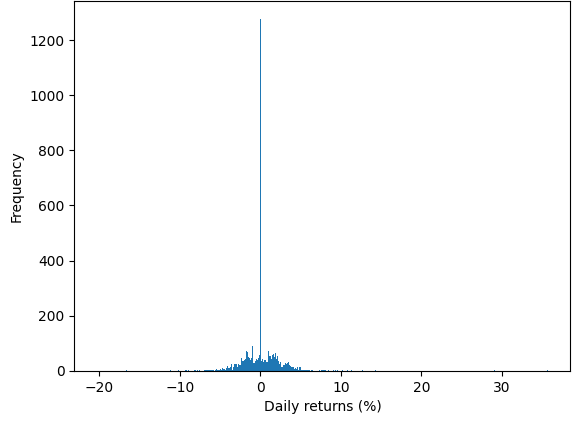
\includegraphics[width=0.80\textwidth]{./assets/Appendices/B/Distribution_DailyReturns/ALI.png}
    \caption{Opening, High, Low, and Closing Prices for ALI}
    \label{fig:returndist_ALI}
\end{figure}
\FloatBarrier

% AP
\begin{figure}[ht]
    \centering
    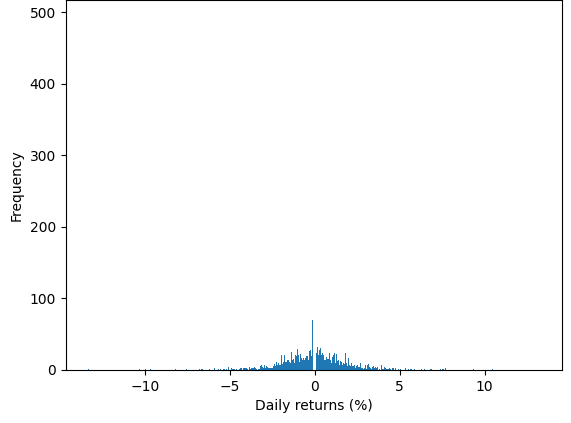
\includegraphics[width=0.80\textwidth]{./assets/Appendices/B/Distribution_DailyReturns/AP.png}
    \caption{Opening, High, Low, and Closing Prices for AP}
    \label{fig:returndist_AP}
\end{figure}
\FloatBarrier

% BDO
\begin{figure}[ht]
    \centering
    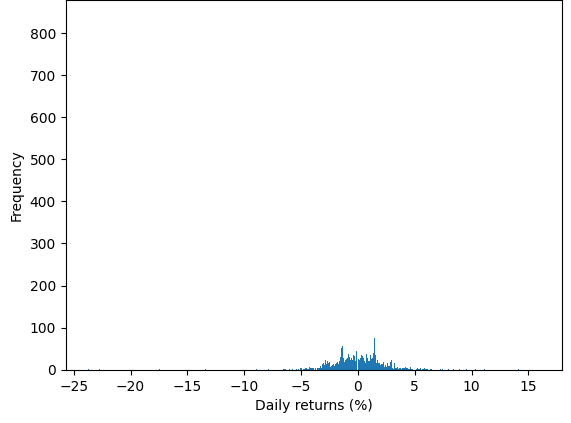
\includegraphics[width=0.80\textwidth]{./assets/Appendices/B/Distribution_DailyReturns/BDO.png}
    \caption{Opening, High, Low, and Closing Prices for BDO}
    \label{fig:returndist_BDO}
\end{figure}
\FloatBarrier

% BLOOM
\begin{figure}[ht]
    \centering
    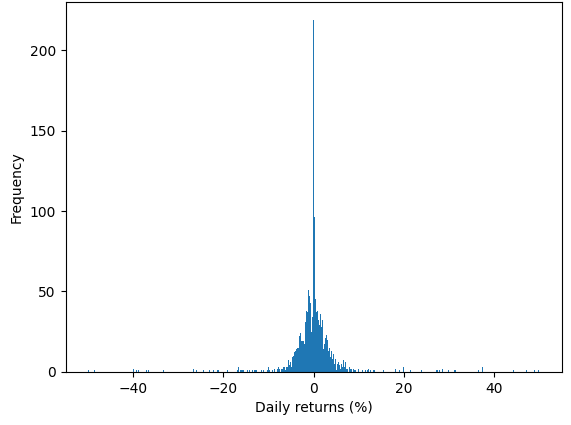
\includegraphics[width=0.80\textwidth]{./assets/Appendices/B/Distribution_DailyReturns/BLOOM.png}
    \caption{Opening, High, Low, and Closing Prices for BLOOM}
    \label{fig:returndist_BLOOM}
\end{figure}
\FloatBarrier

% FGEN
\begin{figure}[ht]
    \centering
    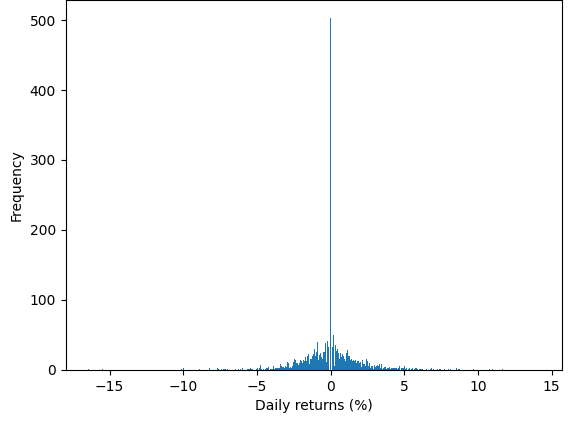
\includegraphics[width=0.80\textwidth]{./assets/Appendices/B/Distribution_DailyReturns/FGEN.png}
    \caption{Opening, High, Low, and Closing Prices for FGEN}
    \label{fig:returndist_FGEN}
\end{figure}
\FloatBarrier

% GLO
\begin{figure}[ht]
    \centering
    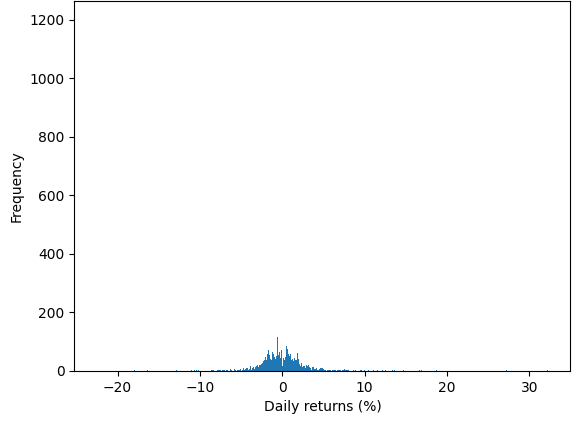
\includegraphics[width=0.80\textwidth]{./assets/Appendices/B/Distribution_DailyReturns/GLO.png}
    \caption{Opening, High, Low, and Closing Prices for GLO}
    \label{fig:returndist_GLO}
\end{figure}
\FloatBarrier

% ICT
\begin{figure}[ht]
    \centering
    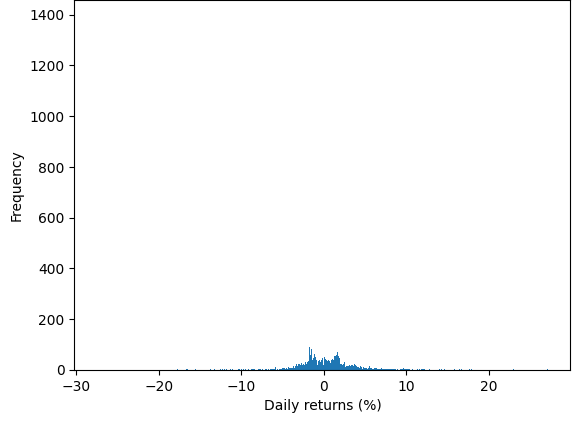
\includegraphics[width=0.80\textwidth]{./assets/Appendices/B/Distribution_DailyReturns/ICT.png}
    \caption{Opening, High, Low, and Closing Prices for ICT}
    \label{fig:returndist_ICT}
\end{figure}
\FloatBarrier

% JGS
\begin{figure}[ht]
    \centering
    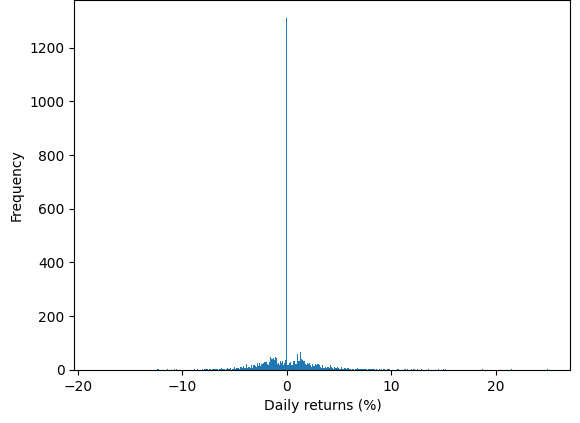
\includegraphics[width=0.80\textwidth]{./assets/Appendices/B/Distribution_DailyReturns/JGS.png}
    \caption{Daily Return Distribution of JGS}
    \label{fig:returndist_JGS}
\end{figure}
\FloatBarrier
    
% LTG
\begin{figure}[ht]
    \centering
    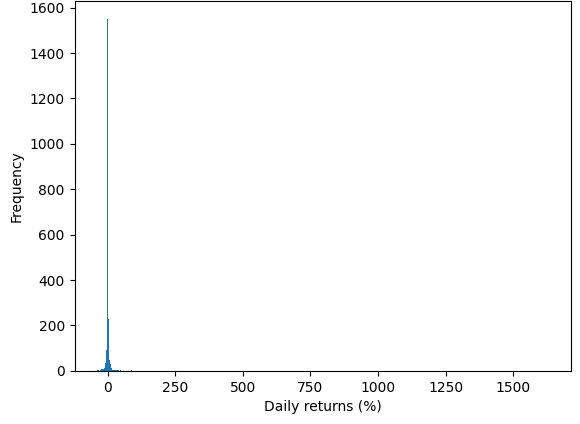
\includegraphics[width=0.80\textwidth]{./assets/Appendices/B/Distribution_DailyReturns/LTG.png}
    \caption{Daily Return Distribution of LTG}
    \label{fig:returndist_LTG}
\end{figure}
\FloatBarrier

% MEG
\begin{figure}[ht]
    \centering
    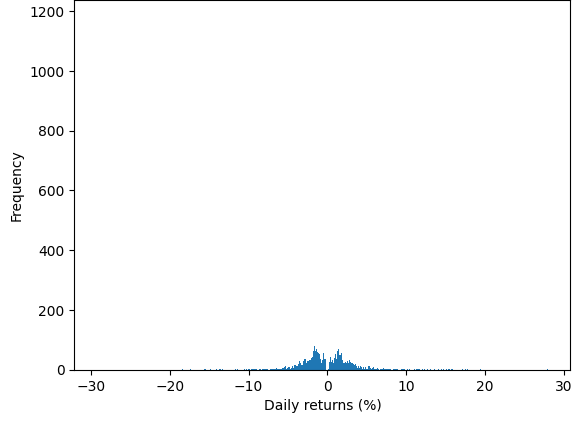
\includegraphics[width=0.80\textwidth]{./assets/Appendices/B/Distribution_DailyReturns/MEG.png}
    \caption{Daily Return Distribution of MEG}
    \label{fig:returndist_MEG}
\end{figure}
\FloatBarrier

% MER
\begin{figure}[ht]
    \centering
    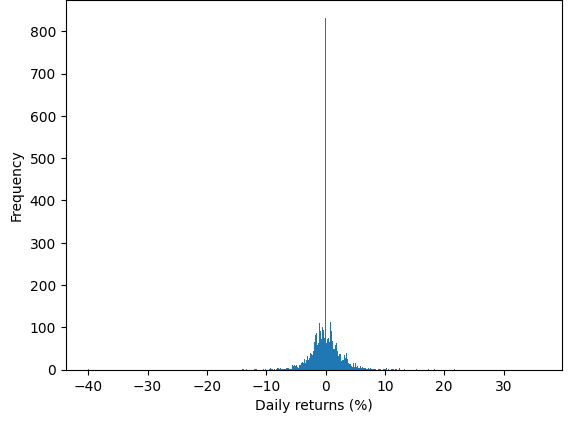
\includegraphics[width=0.80\textwidth]{./assets/Appendices/B/Distribution_DailyReturns/MER.png}
    \caption{Daily Return Distribution of MER}
    \label{fig:returndist_MER}
\end{figure}
\FloatBarrier

% MPI
\begin{figure}[ht]
    \centering
    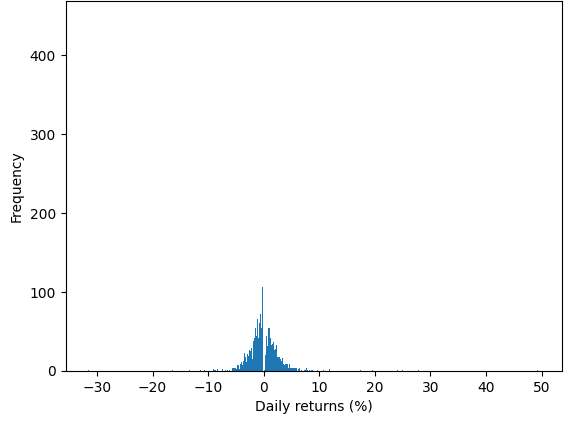
\includegraphics[width=0.80\textwidth]{./assets/Appendices/B/Distribution_DailyReturns/MPI.png}
    \caption{Daily Return Distribution of MPI}
    \label{fig:returndist_MPI}
\end{figure}
\FloatBarrier

% PGOLD
\begin{figure}[ht]
    \centering
    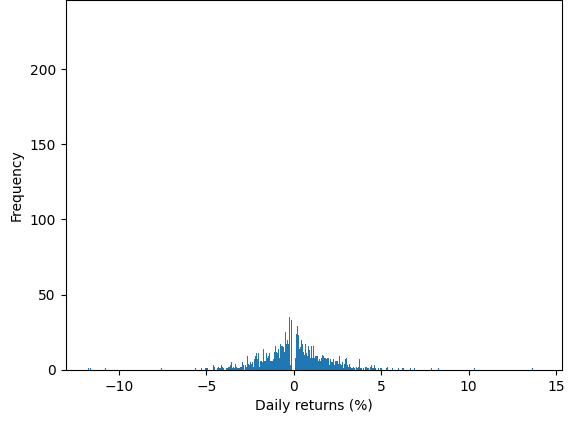
\includegraphics[width=0.80\textwidth]{./assets/Appendices/B/Distribution_DailyReturns/PGOLD.png}
    \caption{Daily Return Distribution of PGOLD}
    \label{fig:returndist_PGOLD}
\end{figure}
\FloatBarrier

% PSEI
\begin{figure}[ht]
    \centering
    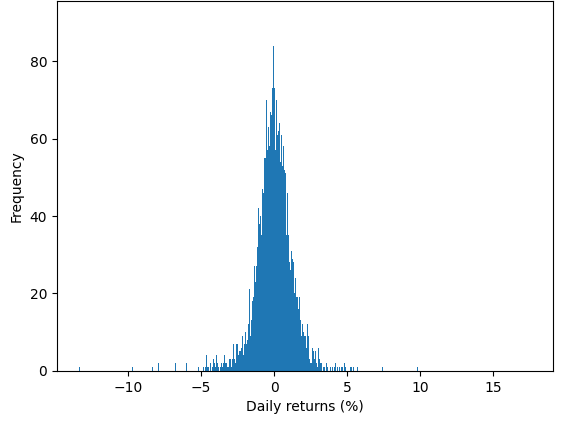
\includegraphics[width=0.80\textwidth]{./assets/Appendices/B/Distribution_DailyReturns/PSEI.png}
    \caption{Daily Return Distribution of PSEI}
    \label{fig:returndist_PSEI}
\end{figure}
\FloatBarrier

% RLC
\begin{figure}[ht]
    \centering
    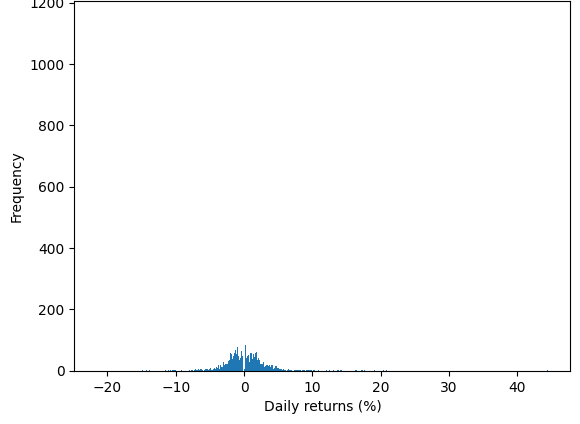
\includegraphics[width=0.80\textwidth]{./assets/Appendices/B/Distribution_DailyReturns/RLC.png}
    \caption{Daily Return Distribution of RLC}
    \label{fig:returndist_RLC}
\end{figure}
\FloatBarrier

% RRHI
\begin{figure}[ht]
    \centering
    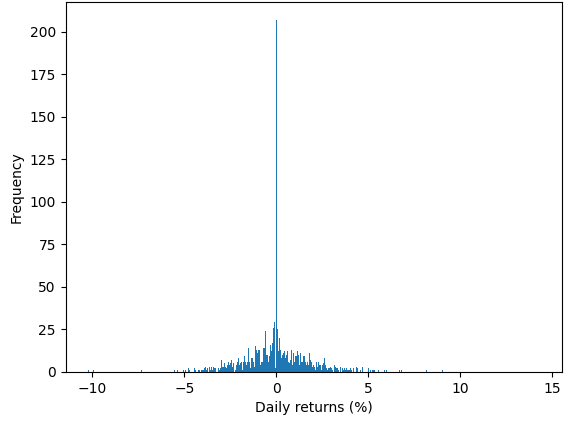
\includegraphics[width=0.80\textwidth]{./assets/Appendices/B/Distribution_DailyReturns/RRHI.png}
    \caption{Daily Return Distribution of RRHI}
    \label{fig:returndist_RRHI}
\end{figure}
\FloatBarrier

% SMC
\begin{figure}[ht]
    \centering
    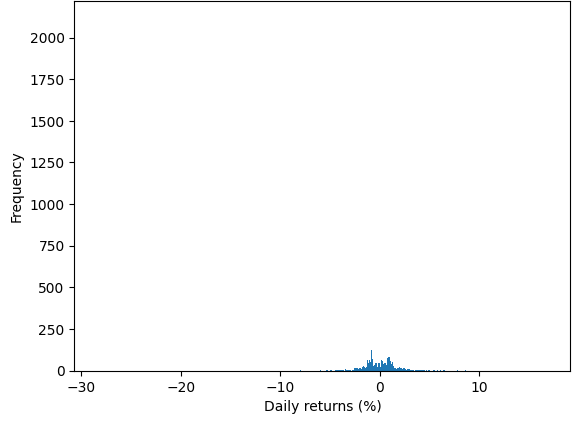
\includegraphics[width=0.80\textwidth]{./assets/Appendices/B/Distribution_DailyReturns/SMC.png}
    \caption{Daily Return Distribution of SMC}
    \label{fig:returndist_SMC}
\end{figure}
\FloatBarrier

% TEL
\begin{figure}[ht]
    \centering
    \includegraphics[width=0.80\textwidth]{./assets/Appendices/B/Distribution_DailyReturns/TEL.png}
    \caption{Daily Return Distribution of TEL}
    \label{fig:returndist_TEL}
\end{figure}
\FloatBarrier

% URC
\begin{figure}[ht]
    \centering
    \includegraphics[width=0.80\textwidth]{./assets/Appendices/B/Distribution_DailyReturns/URC.png}
    \caption{Daily Return Distribution of URC}
    \label{fig:returndist_URC}
\end{figure}
\FloatBarrier

% Raw Risk Profile Scores
\begin{figure}[ht]
    \centering
    \includegraphics[width=0.80\textwidth]{./assets/Appendices/B/Distribution_DailyReturns/Raw_RiskTable.png}
    \caption{Raw Risk Profile Scores}
    \label{fig:rawrisktable}
\end{figure}
\FloatBarrier


\section{Raw alamSYS Test Data}
\label{sec:rawalamSYS}
This section is divided into three sections: raw system logs, PSEI trading baseline data, 
and raw real-world alamSYS application.

\subsection{Raw System Logs}
\label{subsec:rawsyslogs}

% Idle
\begin{figure}[ht]
    \centering
    \includegraphics[height=0.80\textheight]{./assets/Appendices/B/RawTestsData/RawLogs/IdleStats.png}
    \caption{Raw Logs of Idle System Statistics}
    \label{fig:idleStats}
\end{figure}
\FloatBarrier

% Deployment Stress Test
\begin{figure}[ht]
    \centering
    \includegraphics[height=0.80\textheight]{./assets/Appendices/B/RawTestsData/RawLogs/DeploymentStats.png}
    \caption{Raw Logs of Deployment System Statistics}
    \label{fig:deployStats}
\end{figure}
\FloatBarrier

% DCMStats
\begin{figure}[ht]
    \centering
    \includegraphics[height=0.80\textheight]{./assets/Appendices/B/RawTestsData/RawLogs/DCMStats.png}
    \caption{Raw Logs of Data Collector Module (DCM) System Statistics}
    \label{fig:DCMStats}
\end{figure}
\FloatBarrier

% DPMStats
\begin{figure}[ht]
    \centering
    \includegraphics[height=0.80\textheight]{./assets/Appendices/B/RawTestsData/RawLogs/DPMStats.png}
    \caption{Raw Logs of Data Processor Module (DPM) System Statistics}
    \label{fig:DPMStats}
\end{figure}
\FloatBarrier

% PREPROCStats
\begin{figure}[ht]
    \centering
    \includegraphics[height=0.80\textheight]{./assets/Appendices/B/RawTestsData/RawLogs/PREPROCStats.png}
    \caption{Raw Logs of alamPREPROCESSOR System Statistics}
    \label{fig:PreProcStats}
\end{figure}
\FloatBarrier

\subsection{PSEI Trading Baseline Data}
\label{subsec:baseline}

% Day 1
\begin{figure}[ht]
    \centering
    \includegraphics[width=0.45\textwidth]{./assets/Appendices/B/RawTestsData/PSEI_baseline/day1.png}
    \caption{Day 1 PSEI Trading Raw Data}
    \label{fig:PSEIday1}
\end{figure}
\FloatBarrier

% Day 2
\begin{figure}[ht]
    \centering
    \includegraphics[width=0.45\textwidth]{./assets/Appendices/B/RawTestsData/PSEI_baseline/day2.png}
    \caption{Day 2 PSEI Trading Raw Data}
    \label{fig:PSEIday2}
\end{figure}
\FloatBarrier

% Day 3
\begin{figure}[ht]
    \centering
    \includegraphics[width=0.45\textwidth]{./assets/Appendices/B/RawTestsData/PSEI_baseline/day3.png}
    \caption{Day 3 PSEI Trading Raw Data}
    \label{fig:PSEIday3}
\end{figure}
\FloatBarrier

% Day 4
\begin{figure}[ht]
    \centering
    \includegraphics[width=0.45\textwidth]{./assets/Appendices/B/RawTestsData/PSEI_baseline/day4.png}
    \caption{Day 4 PSEI Trading Raw Data}
    \label{fig:PSEIday4}
\end{figure}
\FloatBarrier

% Day 5
\begin{figure}[ht]
    \centering
    \includegraphics[width=0.45\textwidth]{./assets/Appendices/B/RawTestsData/PSEI_baseline/day5.png}
    \caption{Day 5 PSEI Trading Raw Data}
    \label{fig:PSEIday5}
\end{figure}
\FloatBarrier

% Day 6
\begin{figure}[ht]
    \centering
    \includegraphics[width=0.45\textwidth]{./assets/Appendices/B/RawTestsData/PSEI_baseline/day6.png}
    \caption{Day 6 PSEI Trading Raw Data}
    \label{fig:PSEIday6}
\end{figure}
\FloatBarrier

% Day 7
\begin{figure}[ht]
    \centering
    \includegraphics[width=0.45\textwidth]{./assets/Appendices/B/RawTestsData/PSEI_baseline/day7.png}
    \caption{Day 7 PSEI Trading Raw Data}
    \label{fig:PSEIday7}
\end{figure}
\FloatBarrier

% Day 8
\begin{figure}[ht]
    \centering
    \includegraphics[width=0.45\textwidth]{./assets/Appendices/B/RawTestsData/PSEI_baseline/day8.png}
    \caption{Day 8 PSEI Trading Raw Data}
    \label{fig:PSEIday8}
\end{figure}
\FloatBarrier

% Day 9
\begin{figure}[ht]
    \centering
    \includegraphics[width=0.45\textwidth]{./assets/Appendices/B/RawTestsData/PSEI_baseline/day9.png}
    \caption{Day 9 PSEI Trading Raw Data}
    \label{fig:PSEIday9}
\end{figure}
\FloatBarrier

% Day 10
\begin{figure}[ht]
    \centering
    \includegraphics[width=0.45\textwidth]{./assets/Appendices/B/RawTestsData/PSEI_baseline/day10.png}
    \caption{Day 10 PSEI Trading Raw Data}
    \label{fig:PSEIday10}
\end{figure}
\FloatBarrier

\subsection{Raw Real-world alamSYS Application}
\label{subsec:rawalamSYSapp}

\begin{figure}[ht]
    \centering
    \includegraphics[width=0.80\textwidth]{./assets/Appendices/B/RawTestsData/RealWorldApplicationLog.png}
    \caption{Real World Application Raw Data Logs}
    \label{fig:RealWorldApplicationLog}
\end{figure}
\FloatBarrier


\section{Gantt Chart}

% Full Gantt Chart
\begin{figure}[ht]
    \centering
    \includegraphics[width=0.80\textwidth]{./assets/Chapter_3/Gantt/Gantt_Chart_Full.png}
    \caption{Full Gantt Chart}
    \label{fig:gantt_chart_full}
\end{figure}
\FloatBarrier

% Gantt Chart for Sprint 1
\begin{figure}[ht]
    \centering
    \includegraphics[width=0.80\textwidth]{./assets/Chapter_3/Gantt/Gantt_Chart_Sprint1.png}
    \caption{Gantt Chart for Sprint 1}
    \label{fig:gantt_chart_sprint1}
\end{figure}
\FloatBarrier

% Gantt Chart for Sprint 2
\begin{figure}[ht]
    \centering
    \includegraphics[width=0.80\textwidth]{./assets/Chapter_3/Gantt/Gantt_Chart_Sprint2.png}
    \caption{Gantt Chart for Sprint 2}
    \label{fig:gantt_chart_sprint2}
\end{figure}
\FloatBarrier

% Gantt Chart for Sprint 3
\begin{figure}[ht]
    \centering
    \includegraphics[width=0.80\textwidth]{./assets/Chapter_3/Gantt/Gantt_Chart_Sprint3.png}
    \caption{Gantt Chart for Sprint 3}
    \label{fig:gantt_chart_sprint3}
\end{figure}
\FloatBarrier

% Gantt Chart for Sprint 4
\begin{figure}[ht]
    \centering
    \includegraphics[width=0.80\textwidth]{./assets/Chapter_3/Gantt/Gantt_Chart_Sprint4.png}
    \caption{Gantt Chart for Sprint 4}
    \label{fig:gantt_chart_sprint4}
\end{figure}
\FloatBarrier

% Gantt Chart for Sprint 5
\begin{figure}[ht]
    \centering
    \includegraphics[width=0.80\textwidth]{./assets/Chapter_3/Gantt/Gantt_Chart_Sprint5.png}
    \caption{Gantt Chart for Sprint 5}
    \label{fig:gantt_chart_sprint5}
\end{figure}
\FloatBarrier

% Gantt Chart for Sprint 6
\begin{figure}[ht]
    \centering
    \includegraphics[width=0.80\textwidth]{./assets/Chapter_3/Gantt/Gantt_Chart_Sprint6.png}
    \caption{Gantt Chart for Sprint 6}
    \label{fig:gantt_chart_sprint6}
\end{figure}
\FloatBarrier